\documentclass[11pt]{article}%
\usepackage{geometry}%
\geometry{a4paper,
  lmargin=2cm,rmargin=2cm,tmargin=2.5cm,bmargin=2.5cm}

% \input{../macros_Livre.tex}
\input{../macros.tex}

% \renewcommand{\thesection}{\Roman{section}.\hspace{-.3cm}}
% \renewcommand{\thesubsection}{\Alph{subsection}.\hspace{-.2cm}}

\pagestyle{fancy} %
\lhead{ECE2 \hfill Mathématiques \\} %
\chead{\hrule} %
\rhead{} %
\lfoot{} %
\cfoot{} %
\rfoot{\thepage} %

\renewcommand{\headrulewidth}{0pt}% : Trace un trait de séparation
                                    % de largeur 0,4 point. Mettre 0pt
                                    % pour supprimer le trait.

\renewcommand{\footrulewidth}{0.4pt}% : Trace un trait de séparation
                                    % de largeur 0,4 point. Mettre 0pt
                                    % pour supprimer le trait.

\setlength{\headheight}{14pt}

\title{\bf \vspace{-1.6cm} EDHEC 2019} %
\author{} %
\date{} %
\begin{document}

\maketitle %
\vspace{-1.2cm}\hrule %
\thispagestyle{fancy}

\vspace*{.4cm}

%%DEBUT

\section*{Exercice 1}

\noindent
On considère les matrices $A =
\begin{smatrix}
  0 & 1 & 1 \\
  -2 & 3 & 2 \\
  1 & -1 & 0
\end{smatrix}
$ et $I =
\begin{smatrix}
  1 & 0 & 0 \\
  0 & 1 & 0 \\
  0 & 0 & 1
\end{smatrix}
$.\\
On note $f$ l'endomorphisme de $\R^3$ dont $A$ est la matrice
relativement à la base canonique $\B = (e_1, \ e_2, \ e_3)$ de $\R^3$
et $\id$ l'endomorphisme identité de $\R^3$ dont la matrice est $I$.

\begin{noliste}{1.}
  \setlength{\itemsep}{4mm}
\item
  \begin{noliste}{a)}
    \setlength{\itemsep}{2mm}
  \item Déterminer $(A - I)^2$.

    \begin{proof}~%
      \[
      (A - I)^2 \ = \ 
      \begin{smatrix}
        -1 & 1 & 1 \\
        -2 & 2 & 2 \\
        1 & -1 & -1
      \end{smatrix}
      \begin{smatrix}
        -1 & 1 & 1 \\
        -2 & 2 & 2 \\
        1 & -1 & -1
      \end{smatrix}
      \ = \
      \begin{smatrix}
        0 & 0 & 0 \\
        0 & 0 & 0 \\
        0 & 0 & 0 
      \end{smatrix}
      \]
      \conc{$(A - I)^2 = 0_{\M{3}}$}~\\[-1.2cm]
    \end{proof}

  \item En déduire que $A$ est inversible et écrire $A^{-1}$ comme
    combinaison linéaire de $I$ et de $A$.    

    \begin{proof}~%
      \begin{noliste}{$\sbullet$}
      \item Calculons tout d'abord :
        \[
        \begin{array}{C{2cm}rcl@{\qquad}>{\it}R{6cm}}
          & (A - I)^2 & = & A^2 - 2 \, A + I
          & (car la matrice $I$ commute avec $A$, matrice de même ordre)
        \end{array}
        \]

      \item  Ainsi, d'après la question précédente : 
        \[
        \begin{array}{C{2cm}rcl@{\qquad}>{\it}R{5cm}}
          & A^2 - 2 \, A + I & = & 0_{\M{3}}
          \\[.2cm]
          donc & -A^2 + 2 \, A & = & I
          \\[.2cm]
          et & A \, (-A + 2 \, I) & = & I
        \end{array}
        \]
        \conc{On en déduit que $A$ est inversible d'inverse $A^{-1} =
          -A + 2 \, I = 
          \begin{smatrix}
            2 & -1 & -1 \\
            2 & -1 & -2 \\
            -1 & 1 & 2
          \end{smatrix}$.}~\\[-1.4cm]
      \end{noliste}
    \end{proof}

  \end{noliste}

\item On pose $A = N + I$.
  \begin{remarkL}{.72}
    Autrement dit, on note $N \in \M{3}$ la matrice définie par : $N =
    A - I$.
  \end{remarkL}
  \begin{noliste}{a)}
    \setlength{\itemsep}{2mm}
  \item Exprimer pour tout entier naturel $n$, la matrice $A^n$ comme
    combinaison linéaire de $I$ et de $N$ puis l'écrire comme
    combinaison linéaire de $I$ et $A$.

    \begin{proof}~%
      \begin{noliste}{$\sbullet$}
      \item On a démontré en question \itbf{1.a)} : $N^2 = \big( A- I
        \big)^2 = 0_{\M{3}}$.\\[.2cm]
        On en déduit, par une récurrence immédiate, que pour tout $k
        \geq 2$, $N^k = 0_{\M{3}}$.\\
        {\it (ou alors on remarque : $\forall k \geq 2$, $N^k = N^2 \
          N^{k-2} = 0_{\M{3}} \ N^{k-2}= 0_{\M{3}}$)}


        \newpage


      \item Les matrices $I$ et $N$ commutent (car $I$ commute avec
        toutes les matrices du même ordre).

      \item Soit $n \geq 1$. D'après la formule du binôme de Newton :
        \[
	\begin{array}{R{2cm}rcl@{\quad}>{\it}R{5.4cm}}
          & A^{n} & = & (N + I)^n \ = \ \Sum{k=0}{n} \dbinom{n}{k} \
          (I)^{n-k} \ (N)^k   
          \\[.6cm]
          & & = & \Sum{k=0}{n} \dbinom{n}{k} \ I \, N^k \ = \
          \Sum{k=0}{n} \dbinom{n}{k} \ N^k 
          & (car : $\forall j \in \N, \ I^j = I$)
          \nl
          \nl[-.2cm]
          & & = & 
          \Sum{k=0}{1} \dbinom{n}{k} \ N^k +
          \Sum{k=2}{n} \dbinom{n}{k} \ N^k & 
          (ce découpage est \\ valable car $n \geq 1$) 
          \nl
          \nl[-.2cm]
          & & = & 
          \Sum{k=0}{1} \dbinom{n}{k} \ N^k 
          & (car : $\forall k \geq 2, \ N^k = 0_{\M{3}}$)
          \nl
          \nl[-.2cm]
          & & = & \dbinom{n}{0} \ N^0  + \dbinom{n}{1} \ N^1
          \\[.6cm] 
          & & = & I + n \, N
	\end{array}
        \]

      \item De plus : $I - 0 \cdot N = I$ \ et \ $A^0 = I$.\\
        La formule précédente reste valable pour $n = 0$.
      \end{noliste}
      \conc{Ainsi, pour tout $n \in \N$, \ $A^n = I + n \, N$.}
      \begin{remarkL}{.98}%~
        \begin{noliste}{$\sbullet$}
        \item La \og relation de Chasles \fg{} stipule que pour tout
          $(m, p, n) \in \N^3$ tel que $m \leq p \leq n$ :
          \[
          \Sum{k = m}{n} u_k = \Sum{k = m}{p} u_k + \Sum{k = p+1}{n}
          u_k
          \]
          {\it (la somme la plus à droite est nulle si $p = n$)}\\
          où $(u_n)$ est une suite quelconque de réels ou de matrices.
          % On insiste ici sur le fait que cette relation n'est
          % vérifiée que sous la condition $m \leq p \leq n$.
        \item Dans cette question, on est dans le cas où $m = 0$ et $p
          = 1$.\\
          L'argument $n \geq 1$ est donc essentiel pour découper la
          somme.\\
          % :
          % \[
          % \Sum{k = 0}{n} u_k = \Sum{k = 0}{0} u_k + \Sum{k = 1}{n}
          % u_k
          % \]
          Le cas $n = 0$ doit donc être traité à part.
        \item Ici, la matrice $N$ vérifie : $\forall k \geq 2, \ N^k =
          0_{\M{3}}$. Elle est dite nilpotente d'indice $2$ (ce terme
          n'est pas au programme et il est préférable de ne pas
          l'utiliser dans une copie). Si elle avait été nilpotente
          d'ordre $3$, il aurait fallu traiter à part les cas $n = 0$
          et $n = 1$ (le découpage de la somme est alors valable pour
          $n \geq 2$).
        \end{noliste}
      \end{remarkL}%~\\[-1.4cm]
      \begin{noliste}{$\sbullet$}
      \item Enfin, pour tout $n \in \N$ :
        \[
        A^{n} \ = \ I + n \, N \ = \ I + n \, (A - I) \ = \ (1 - n) \,
        I + n \, A
        \]
        \conc{$\forall n \in \N$, $A^{n} \ = \ (1 - n) \, I + n \,
          A$}~\\[-1.4cm] 
      \end{noliste}
    \end{proof}


    \newpage


  \item Vérifier que l'expression précédente est aussi valable pour
    $n=-1$.

    \begin{proof}~\\%
      \begin{noliste}{$\sbullet$}
      \item Tout d'abord : $A^{-1} = 2 \, I - A$ d'après la question
        \itbf{1.b)}.
      \item D'autre part : $(1 - (-1)) \, I + (-1) \, A = 2 \, I - A$.        
      \end{noliste}
      \conc{La formule précédente est aussi valable pour $n =
        -1$.}~\\[-1.2cm] 
    \end{proof}
   \end{noliste}

\item 
  \begin{noliste}{a)}
    \setlength{\itemsep}{2mm}
  \item Utiliser la première question pour déterminer la seule valeur
    propre de $A$.

    \begin{proof}~%
      \begin{noliste}{$\sbullet$}
      \item D'après la question précédente, le polynôme $Q(X) = (X -
        1)^2$ est un polynôme annulateur de la matrice $A$. Ainsi :
        $\spc(A) \subset \{\text{racines de $Q$}\} = \{0\}$.%
      \end{noliste}
      \conc{Ainsi : $\spc(A) \subset \{ 1 \}$ et $1$ est l'unique
        valeur propre possible de $A$.}
      \begin{remarkL}{.98}
        \begin{noliste}{$\sbullet$}
        \item Une matrice $A\in \M{n}$ possède {\tt TOUJOURS} un
          polynôme annulateur non nul $Q$.\\
          On peut même démontrer (ce n'est pas au programme en ECE)
          qu'il existe toujours un tel polynôme de degré (au plus)
          $n$.
	    
        \item Si $Q$ est un polynôme annulateur de $A$ alors, pour
          tout $\alpha \in \R$, le polynôme $\alpha \, Q$ est toujours
          un polynôme annulateur de $A$ puisque :
          \[
          (\alpha \, Q)(A) \ = \ \alpha \, Q(A) \ = \ 0_{\M{n}}
          \]
          Cela suffit à démontrer que $A$ possède une infinité de
          polynômes annulateurs.\\
          On peut en obtenir d'autres. Par exemple $R(X) = (X-5) \,
          Q(X)$ est un polynôme annulateur de $A$ puisque :
          \[
          R(A) \ = \ (A-5 \, I) \, Q(A) \ = \ 0_{\M{n}}
          \]
          Il faut donc parler {\tt D'UN} polynôme annulateur d'une
          matrice.
          
        \item Les racines d'un polynôme annulateur ne sont pas
          forcément toutes valeurs propres de $A$. Si c'était le
          cas, $A$ aurait une infinité de valeurs propres (elle en
          possède au plus $n$). Par exemple, comme $R(X) = (X-5) \,
          Q(X)$ est un polynôme annulateur, un tel raisonnement
          permettrait de démontrer que $5$ est aussi valeur propre.
        \end{noliste}
      \end{remarkL}
      \begin{noliste}{$\sbullet$}
      \item Démontrons que $2$ est valeur propre de $A$.
        \[
        A - I \ = \
        \begin{smatrix}
          -1 & 1 & 1 \\
          -2 & 2 & 2 \\
          1 & -1 & -1
        \end{smatrix}
        \]
        Cette matrice est non inversible car possède $2$ colonnes
        colinéaires ($C_2 = - C_1$).%
        \conc{On en déduit que $1$ est l'unique valeur propre de
          $A$.}~\\[-1.5cm] 
      \end{noliste}      
    \end{proof}


    \newpage


  \item En déduire si $A$ est ou n'est pas diagonalisable.

    \begin{proof}~\\%
      Démontrons que $A$ n'est pas diagonalisable. On procède par
      l'absurde.\\
      Supposons que $A$ est diagonalisable.\\
      Il existe donc une matrice inversible $P \in \M{3}$ et une
      matrice diagonale $D \in \M{3}$ dont les coefficients diagonaux
      sont les valeurs propres de $A$ telles que $A = PDP^{-1}$.\\
      Or $1$ est la seule valeur propre de $A$. Ainsi $D = I$ et :
      \[
      T \ = \ P \, I_3 \, P^{-1} \ = \ P \, I_3 \, P^{-1} \ = \ I_3
      \]
      Absurde ! %      
      \conc{La matrice $A$ n'est pas diagonalisable.}~\\[-1.2cm]
    \end{proof}

  \end{noliste}

\item On pose $u_1 = (f - \id)(e_1)$ et $u_2 = e_1 + e_3$.
  \begin{noliste}{a)}
    \setlength{\itemsep}{2mm}
  \item Montrer que le rang de $f - \id$ est égal à $1$.

    \begin{proof}~%
      \[
      \begin{array}{rcl@{\qquad}>{\it}R{5cm}}
        \rg(f - \id) & = & \rg(A - I)
        \\[.2cm]
        & = &
        \rg\left( 
          \begin{smatrix}
            -1 & 1 & 1 \\
            -2 & 2 & 2 \\
            1 & -1 & -1
          \end{smatrix}
        \right) 
        \\[.6cm]
        & = & 
        \rg\left( 
          \begin{smatrix}
            -1 \\
            -2 \\
            1 
          \end{smatrix},
          \begin{smatrix}
            1 \\
            2 \\
            -1 
          \end{smatrix},
          \begin{smatrix}
            1 \\
            2 \\
            -1 
          \end{smatrix}
        \right) 
        %\\[1cm]
        %& = & 
        \ = \ 
        \rg\left( 
          \begin{smatrix}
            1 \\
            2 \\
            -1 
          \end{smatrix}
        \right) 
        \ = \ 1
      \end{array}
      \]
      La dernière égalité est vérifié car la famille $\left( 
          \begin{smatrix}
            1 \\
            2 \\
            -1 
          \end{smatrix}
        \right)$ est libre (constituée uniquement d'un vecteur non
        nul).%
        \conc{Ainsi : $\rg(f - \id) = 1$.}~\\[-1cm]
    \end{proof}

  \item Justifier que $(u_1, u_2)$ est une base de $\kr(f - \id)$.

    \begin{proof}~\\%
      Notons $E_1 = \Mat_{\B}(e_1) =
      \begin{smatrix}
        1 \\
        0 \\
        0
      \end{smatrix}
      $, $E_3 = \Mat_{\B}(e_2) =
      \begin{smatrix}
        0 \\
        0 \\
        1
      \end{smatrix}
      $ et $U_1 = \Mat_{\B}(u_1)$,  $U_2 = \Mat_{\B}(u_2)$.
      \begin{noliste}{$\sbullet$}
      \item Remarquons tout d'abord :
        \[
        \begin{array}{rcl@{\qquad}>{\it}R{5cm}}
          \Mat_{\B}(u_1) & = & \Mat_{\B}\Big( (f - \id) (e_1) \Big)
          \\[.4cm]
          & = & \Mat_{\B}\big( f - \id \big) \times \Mat_{\B}( e_1 )
          \\[.4cm]
          & = & \big(\Mat_{\B}(f) - \Mat_{\B}(\id) \big) \times
          \Mat_{\B}( e_1 ) 
          & (par linéarité de $f$)
          \nl
          \nl[-.2cm]
          & = & \big( A - I \big) \ E_1 \ = \ 
          \begin{smatrix}
            -1 & 1 & 1 \\
            -2 & 2 & 2 \\
            1 & -1 & -1
          \end{smatrix}
          \begin{smatrix}
            1 \\
            0 \\
            0
          \end{smatrix}
          \\[.4cm] 
          & = &
          \begin{smatrix}
            -1 \\
            -2 \\
            1
          \end{smatrix}        
          \ = \ \Mat_{\B}\big( (-1, -2, 1) \big)
        \end{array}
        \]
        \conc{Par isomorphisme de représentation, $u_1 = (-1, -2, 1)$.}


        \newpage


        \noindent
        Puis : $\Mat_{\B}\Big( (f - \id) (u_1) \Big) \ = \ \big( A - I
        \big) \ U_1 \ = \
        \begin{smatrix}
          -1 & 1 & 1 \\
          -2 & 2 & 2 \\
          1 & -1 & -1
        \end{smatrix}
        \begin{smatrix}
          -1 \\
          -2 \\
          1
        \end{smatrix}
        \ = \
        \begin{smatrix}
          0 \\
          0 \\
          0
        \end{smatrix}
        = \Mat_{\B}\big( (0, 0, 0) \big) $.%
        \conc{Ainsi : $(f - \id)(u_1) = 0_{\R^3}$, c'est-à-dire : $u_1
          \in \kr(f - \id)$.}
        \begin{remarkL}{.98}
          On pouvait ici opter pour une présentation plus élégante :
          \[
          \begin{array}{rcl@{\qquad}>{\it}R{5cm}}
            (f - \id) \, (u_1) & = & (f - \id) \, \Big( (f - \id) (e_1)
            \Big)
            \\[.2cm]
            & = & (f - \id)^2 \, (e_1) \ = \ 0_{\R^3}
            & (car $(f - \id)^2 \ = \ 0_{\LL{\R^3}}$ puisque $(A-I)^2 =
            0_{\M{3}}$) 
          \end{array}
          \]
          La présentation choisie est plus calculatoire. Cela a un
          intérêt : on obtient la valeur de $u_1$.
        \end{remarkL}

      \item Ensuite : 
        \[
        \begin{array}{rcl@{\qquad}>{\it}R{2.5cm}}
          \Mat_{\B}\big( (f - \id)(u_2) \big) & = & 
          \Mat_{\B}\big(f - \id \big) \times \Mat_{\B}\big(u_1 \big)
          \\[.4cm]
%           & = & 
%           \Mat_{\B}\big(f - \id \big) \times \Mat_{\B}\big(e_1 + e_3
%           \big)
%           \\[.2cm]
%           & = &
%           \big(\Mat_{\B}(f) - \Mat_{\B}(\id) \big) \times \big(
%           \Mat_{\B}(e_1) + \Mat_{\B}(e_3) \big)
%           & (par linéarité de $\Mat_{\B}$)
%           \nl
%           \nl[-.2cm]
          & = & 
          (A - I) \, (E_1 + E_3)
          \\[.4cm]
          & = & 
          \begin{smatrix}
            -1 & 1 & 1 \\
            -2 & 2 & 2 \\
            1 & -1 & -1
          \end{smatrix}
          \begin{smatrix}
            1 \\
            0 \\
            1
          \end{smatrix}
          \ = \ 
          \begin{smatrix}
            0 \\
            0 \\
            0
          \end{smatrix}
          \ = \ \Mat_{\B}\big( (0, 0, 0) \big)
        \end{array}
        \]
        On en déduit, par isomorphisme de représentation : $(f -
        \id)(u_2) = 0_{\R^3}$.%
        \conc{ Ainsi : $u_2 \in \kr(f - \id)$.}
        \begin{remarkL}{.98}%
          \begin{noliste}{$\sbullet$}
          \item L'énoncé ne donne pas directement accès à $f$ mais à
            $A$, sa matrice représentative dans la base $\B$. La base
            $\B$ étant fixée, l'application $\Mat_{\B}(.)$, appelée
            parfois isomorphisme de représentation, permet de traduire
            les propriétés énoncées dans le monde des espaces
            vectoriels en des propriétés énoncées dans le monde
            matriciel.\\
            Voici quelques correspondances dans le cas général :
            \[
            \begin{array}{L{6cm}cR{7cm}}
              $E$ espace vectoriel de dimension $n$ & \longleftrightarrow &
              $\M{n,1}$
              \nl
              \nl[-.2cm]
              $f : E \to E$ endomorphisme & \longleftrightarrow &
              $\Mat_{\B}(f) \in \M{n}$
              \nl
              \nl[-.2cm]
              $f$ bijectif & \longleftrightarrow & $\Mat_{\B}(f)$ inversible
            \end{array}
            \]
            Ou encore, dans le cas précis de l'exercice :
            \[
            \begin{array}{L{6cm}cR{7cm}}
              $f$ & \longleftrightarrow & $A$
              \nl
              \nl[-.2cm]
              $f - \id$ & \longleftrightarrow & $A - I$
              \nl
              \nl[-.2cm]
              $(f - \id)(u_2) = 0_{\R^3}$ & \longleftrightarrow & $(A
              - I) \times U_2 = 0_{\M{3, 1}}$
            \end{array}
            \]
            Il est très fréquent que les énoncés de concours requièrent de
            savoir traduire une propriété d'un monde à l'autre. Il est
            donc indispensable d'être à l'aise sur ce mécanisme.
          \end{noliste}
        \end{remarkL}
        
      \item Enfin, par théorème du rang :
        \[
        \begin{array}{ccccc}
          \dim\big( \R^3 \big) & = & \dim\Big( \kr\big( f - \id
          \big) \Big) & + & \rg\big( f - \id \big) 
          \\[.2cm]
          \shortparallel & & & & \shortparallel
          \\[.2cm]
          3 & & & & 1
        \end{array}
        \]
        On en déduit : $\dim\big( \kr\big( f - \id \big) \big) \ = \ 3
        - 1 \ = \ 2$.%
        \conc{$\dim\big( \kr\big( f - \id \big) \big) \ = \ 2$}

      \item La famille ${\cal F} = (u_1, u_2)$ est :
        \begin{noliste}{$\stimes$}
        \item libre car constituée de deux vecteurs non colinéaires
          ($(-1, -2, 1)$ et $(1, 0, 1)$).

        \item de cardinal $\Card\big( {\cal F} \big) = 2 = \dim\big(
          \kr\big( f - \id \big) \big)$.          
        \end{noliste}
        \conc{On en déduit que la famille ${\cal F}$ est une base de
          $\kr \big(f - \id \big)$.}
      \end{noliste}
      \begin{remark}
        \begin{noliste}{$\sbullet$}
        \item On peut aussi déterminer le noyau de $f - \id$ par
          résolution de systèmes.\\
          Détaillons cette méthode.
        \item Soit $u = (x, y, z) \in \R^3$. Notons $U = \Mat_\B(u) =
          \begin{smatrix}
            x\\
            y\\
            z
          \end{smatrix}$.
          \[
          \begin{array}{rcl}
            u \in \kr\big( f-\id \big) & \Longleftrightarrow & \big(f
            - \id \big) (u) = 0_{\R^3}
            \\[.2cm]
            & \Longleftrightarrow & (A-I) \, U = 0_{\M{3,1}}
            \\[.2cm]
            & \Longleftrightarrow & 
            \begin{smatrix}
              -1 & 1 & 1 \\
              -2 & 2 & 2 \\
              1 & -1 & -1
            \end{smatrix}
            \,
            \begin{smatrix}
              x \\
              y \\
              z
            \end{smatrix}
            =
            \begin{smatrix}
              0 \\
              0 \\
              0
            \end{smatrix}
            \\[.6cm]
            & \Longleftrightarrow &
            \left\{
              \begin{array}{rcrcrcr}
                - \, x & + & y & + & z & = & 0 \\
                - 2 \, x & + & 2\, y & + & 2 \, z & = & 0 \\
                x & - & y & - & z & = & 0 
              \end{array}
            \right.
            \\[.8cm]
            & 
            \begin{arrayEq}
              L_2 \leftarrow L_2 - 2 \, L_1 \\
              L_3 \leftarrow L_3 + L_1
            \end{arrayEq}
            &
            \left\{
              \begin{array}{rcrcrcr}
                - \, x & + & y & + & z & = & 0 \\
                & & & & 0 & = & 0 \\
                & & & & 0 & = & 0
              \end{array}
            \right.
            \\[.8cm]
            & 
            \Longleftrightarrow
            &
            \left\{
              \begin{array}{rcrcr}
                x & = & y & + & z 
              \end{array}
            \right.
          \end{array}
          \]
          Finalement, on obtient l'expression de $\kr(f)$ suivante :
          \[
          \begin{array}{rcl}
            \kr\big( f-\id \big) & = &  \{ (x, \, y, \, z) \in \R^3 \
            | \ x = y + z \}
            \\[.2cm]
            & = &  \{(y+z, y, z) \ | \ (y, z) \in \R^2 \}
            \\[.2cm]
            & = &  \{ y \cdot (1, \, 1, \, 0) + z \cdot (1, \, 0, \,
            1) + \ | \ (y, z) \in \R^2 \}
            \\[.2cm]
            & = & \Vect{(1, 1, 0), (1, 0, 1)}
          \end{array}
          \]

        \item On remarque que la famille génératrice trouvée n'est pas
          celle qui est présente dans l'énoncé. Cependant, comme :
          $(-1, -2, 1) = -2 \cdot (1, 1, 0) + (1, 0, 1)$, on a :
          \[
          \Vect{(1, 1, 0), (1, 0, 1)} \ = \ \Vect{(-1, -2, 1), (1, 0,
            1)} \ = \ \Vect{u_1, u_2}
          \]

%         \item Il faut s'habituer à déterminer les ensembles $E_\lambda(A)$
%         par lecture de la matrice $A - \lambda \, I$.

%       \item Illustrons la méthode avec la matrice de l'exercice et
%         $\lambda = \frac{1}{2}$.\\
%         On cherche les vecteurs $X =
%         \begin{smatrix}
%           x \\
%           y \\
%           z
%         \end{smatrix}
%         $ de $E_{\frac{1}{2}}(A) $ c'est-à-dire les vecteurs tels que
%         : \\
%         $(A - \frac{1}{2} \, I_3) \, X = 0_{\M{3,1}}$. Or :\\[-.1cm]
%         \[
%         \begin{array}{rcl}
%           \begin{smatrix}
%             \frac{1}{2} & -1 & 1 \\
%             0 & 0 & 0 \\
%             0 & 0 & \frac{3}{2}
%           \end{smatrix}
%           \begin{smatrix}
%             x \\
%             y \\
%             z 
%           \end{smatrix}
%           & = & x \cdot C_1 + y \cdot C_2 + z \cdot C_3
%           \\[-.2cm]
%           & = & 
%           x \cdot
%           \begin{smatrix}
%             \frac{1}{2} \\
%             0 \\
%             0
%           \end{smatrix}
%           + y \cdot
%           \begin{smatrix}
%             -1 \\
%             0 \\
%             0 
%           \end{smatrix}
%           + z \cdot
%           \begin{smatrix}
%             1 \\
%             0 \\
%             \frac{3}{2}
%           \end{smatrix}
%         \end{array}
%         \]~\\[-.6cm]
%         Pour obtenir le vecteur $
%         \begin{smatrix}
%           0 \\
%           0 \\
%           0
%         \end{smatrix}
%         $ à l'aide de cette combinaison linéaire, on doit forcément
%         choisir $z = 0$. En effet, si $z$ est non nul, les
%         coefficients en $\eme{2}$ et $\eme{3}$ position de la
%         combinaison linéaire sont non nuls. On prend alors $z = 0$.\\
%         La combinaison linéaire restante est nulle si $\frac{1}{2} \,
%         x - y = 0$, c'est-à-dire si $x = 2y$.\\
%         En prenant par exemple $y = 1$, on obtient : $
%         E_{\frac{1}{2}}(A) \ \supset \ \Vect{
%           \begin{smatrix}
%             2 \\
%             1 \\
%             0 
%           \end{smatrix}
%         } $.\\
%         Et l'égalité est vérifiée car ces deux espaces vectoriels sont
%         de même dimension.

        \end{noliste}
      \end{remark}~\\[-1.4cm]
    \end{proof}
  \end{noliste}


\newpage


\item 
  \begin{noliste}{a)}
    \setlength{\itemsep}{2mm}
  \item Montrer que la famille $(u_1, u_2, e_1)$ est une base de $\R^3$.

    \begin{proof}~
      \begin{noliste}{$\sbullet$}
      \item Montrons que la famille $(u_1, u_2, e_1)$ est libre.\\
	Soit $(\lambda_1, \lambda_2, \lambda_3) \in \R^3$.\\
        Supposons : $\lambda_1 \cdot u_1 +\lambda_2 \cdot u_2 +
        \lambda_3 \cdot e_1 \ = \ 0_{\R^3}$ $(*)$.
        \begin{noliste}{$\stimes$}
        \item Par linéarité de $f-\id$, on obtient, en appliquant
          $f-\id$ de part et d'autre de l'égalité :
          \[
          \begin{array}{ccc}
            \lambda_1 \cdot \bcancel{(f-\id)(u_1)} + \lambda_2 \cdot
            \bcancel{(f-\id)(u_2)} + \lambda_3 \cdot (f-\id)(e_1) & =
            & (f-\id)\big( 0_{\R^3} \big) 
            \\[.2cm]
            \shortparallel & & \shortparallel
            \\[.2cm]
            \lambda_3 \cdot u_1 & & 0_{\R^3}
          \end{array}
          \]
%           \begin{noliste}{$\stimes$}
%           \item 
          En effet, comme $u_1$ et $u_2$ sont deux éléménts de
          $\kr\big( f-\id \big)$ alors : 
          \[
          (f-\id)(u_1) \ = \ 0_{\R^3} \ = \ (f-\id)(u_2)
          \]
%           \item $(f-\id) (e_1) = u_1$ par définition.
%           \end{noliste}
          \conc{Comme $\lambda_3 \cdot u_1 = 0_{\R^3}$ \ et \ $u_1
            \neq 0_{\R^3}$, alors : $\lambda_3 = 0$.}

        \item L'égalité $(*)$ se réécrit alors : $\lambda_1 \cdot
          u_1 + \lambda_2 \cdot u_2 = 0_{\R^3}$.\\
          Or, d'après la question précédente, la famille $(u_1, u_2)$
          est libre.%
          \conc{On en déduit : $\lambda_1 = \lambda_2 = 0$.}
        \end{noliste}
        \conc{Finalement, $\lambda_1 = \lambda_2 = \lambda_3 = 0$ et
          la famille $(u_1, u_2, e_1)$ est bien libre.}
        \begin{remark}
          \begin{noliste}{$\sbullet$}
          \item Il était une nouvelle fois possible de procéder par
            résolution de système. \\
            Détaillons ce point.
          \item Montrons que la famille $(u_1, u_2, e_1)$ est libre.\\
            Soit $(\lambda_1, \lambda_2, \lambda_3) \in
            \R^3$. Supposons : $\lambda_1 \cdot u_1 +\lambda_2 \cdot
            u_2 + \lambda_3 \cdot e_1 \ = \ 0_{\R^3}$.\\[.2cm]
            Les équivalences suivantes sont vérifiées.
            \[
            \begin{array}{cl@{\qquad}>{\it}R{3cm}}
              & \lambda_1 \cdot u_1 + \lambda_2 \cdot u_2 + \lambda_3 \cdot 
              e_1 = 0_{\R^3} 
              \\[.2cm]
              \Longleftrightarrow & \lambda_1 \cdot (-1, -2, 1) + \lambda_2
              \cdot (1, 0, 1) + \lambda_3 \cdot (1, 0, 0) = 0_{\R^3} 
              \\[.2cm]
              \Longleftrightarrow &  
              (-\lambda_1 + \lambda_2 + \lambda_3, \ -\lambda_2, \
              \lambda_1 + \lambda_2) \ = \ (0, 
              0, 0)  
              \\[.2cm]
              \Longleftrightarrow &
              \left\{
                \begin{array}{rcrcrcl}
                  - \lambda_1 & + & \lambda_2 & + & \lambda_3 & = & 0 \\
                  & - & 2 \, \lambda_2 & & & = & 0 \\
                  \lambda_1 & + & \lambda_2 & & & = & 0 
                \end{array}
              \right.
              \\[.8cm]            
              \begin{arrayEq}
                L_3 \leftarrow L_3 + L_1
              \end{arrayEq}
              &  
              \left\{
                \begin{array}{rcrcrcl}
                  - \lambda_1 & + & \lambda_2 & + & \lambda_3 & = & 0 \\
                  & - & 2 \, \lambda_2 & & & = & 0 \\
                  & & 2 \, \lambda_2 & + & \lambda_3 & = & 0 
                \end{array}
              \right.
              \\[.8cm]            
              \begin{arrayEq}
                L_3 \leftarrow L_3 + L_2
              \end{arrayEq}
              &  
              \left\{
                \begin{array}{rcrcrcl}
                  - \lambda_1 & + & \lambda_2 & + & \lambda_3 & = & 0 \\
                  & - & 2 \, \lambda_2 & & & = & 0 \\
                  & & & & \lambda_3 & = & 0 
                \end{array}
              \right.
              \\[.8cm]
              \Longleftrightarrow &  
              \left\{
                \lambda_1 = \lambda_2 = \lambda_3 = 0
              \right.
              \\[.2cm]
              & \text{\it (par remontées successives)}
            \end{array}
            \]
            \conc{Ainsi, $(u_1, u_2, e_1)$ est une famille libre de
              $\R^3$.}
          \end{noliste}
        \end{remark}


        \newpage


      \item On a alors :
	\begin{noliste}{$\stimes$}
        \item la famille $(u_1, u_2, e_1)$ est une famille libre,
        \item $\Card\big( (u_1, u_2, e_1) \big) = 3 = \dim(\R^3)$.
	\end{noliste}
      \end{noliste}
      \conc{Ainsi, $(u_1, u_2, e_1)$ est une base de $\R^3$.}
      \begin{remarkL}{.98}%~
        \begin{noliste}{$\sbullet$}
        \item Le terme {\bf cardinal} est réservé aux ensembles
          finis. La famille $(u_1, u_2, e_1)$ est un ensemble qui
          contient $3$ vecteurs. Elle est donc finie, de cardinal $3$
          (ce qu'on note $\Card((u_1, u_2, e_1)) = 3$).

        \item $\Vect{u_1, u_2, e_1}$ est l'espace vectoriel constitué
          de toutes les combinaisons linéaires des vecteurs $(u_1,
          u_2, e_1)$. C'est un ensemble {\bf infini} de vecteurs, on
          ne peut parler de son cardinal. Par contre, si l'on dispose
          d'une base $(u_1, u_2, e_1)$ d'un espace vectoriel, tout
          vecteur se décompose de manière unique sur cette base. Ceci
          permet de donner une représentation finie de cet ensemble
          infini.

        \item Les notations : $\bcancel{\Card\big( \Vect{u_1, u_2,
              e_1} \big)}$ et $\bcancel{\dim((u_1, u_2, e_1))}$ n'ont
          aucun sens !
        \end{noliste}
      \end{remarkL}~\\[-1.4cm]
    \end{proof}

  \item Déterminer la matrice $T$ de $f$ dans cette même base.

    \begin{proof}~%
      \begin{noliste}{$\sbullet$}
      \item $f(u_1) = 1 \cdot u_1 + 0 \cdot u_2 + 0 \cdot e_1$ \ car \
        $u_1 \in \kr(f - \id) = E_1(f)$.%
        \conc{Ainsi : $\Mat_{(u_1, u_2, e_1)} \big( f(u_1) \big) =
          \begin{smatrix}
            1 \\
            0 \\
            0
          \end{smatrix}
          $.}       

      \item $f(u_2) = 0 \cdot u_1 + 1 \cdot u_2 + 0 \cdot e_1$ \ car \
        $u_2 \in \kr(f - \id) = E_1(f)$.%
        \conc{Ainsi : $\Mat_{(u_1, u_2, e_1)} \big( f(u_2) \big) =
          \begin{smatrix}
            0 \\
            1 \\
            0
          \end{smatrix}
          $.}       

      \item Rappelons que par définition : $u_1 \ = \ (f - \id)(e_1)
        \ = \ f(e_1) - e_1$.\\
        On en déduit : $f(e_1) = 1 \cdot u_1 + 0 \cdot u_2 + 1 \cdot
        e_1$.%
        \conc{Ainsi : $\Mat_{(u_1, u_2, e_1)} \big( f(e_1) \big) =
          \begin{smatrix}
            1 \\
            0 \\
            1
          \end{smatrix}
          $.}       
      \end{noliste}
      \conc{Finalement : $\Mat_{(u_1, u_2, e_1)} (f) =
        \begin{smatrix} 
          1 & 0 & 1 \\
          0 & 1 & 0 \\
          0 & 0 & 1
        \end{smatrix} = T
        $.}%~\\[-1cm]
    \begin{remarkL}{.98}%
      \begin{noliste}{$\sbullet$}
      \item Rappelons tout d'abord que déterminer la matrice
        représentative de $f$ dans la base $(u_1, u_2, e_1)$ consiste
        à exprimer l'image par $f$ des vecteurs $u_1$, $u_2$, $e_1$
        suivant cette même base $(u_1, u_2, e_1)$.

      \item Pour résoudre la question, on se sert ici une nouvelle
        fois de la correspondance entre le monde des espaces
        vectoriels et le monde matriciel.\\
        Ou peut ajouter la correspondance suivante à celle déjà
        évoquée :
        \[
        \begin{array}{L{6.7cm}cR{7cm}}
          expression de $f(u_1)$ dans $(u_1, u_2, e_1)$ &
          \longleftrightarrow & expression de $A U_1$ dans $(U_1, U_2, E_1)$
        \end{array}
        \]
      \end{noliste}
    \end{remarkL}


    \newpage


    \begin{remarkL}{.98}%
      \begin{noliste}{$\sbullet$}
      \item Comme on l'a vu dans la question \itbf{3.b)},
        l'endomorphisme $f$ n'est pas diagonalisable. Il n'existe donc
        pas de base dans laquelle la matrice représentant $f$ est
        diagonale.

      \item Dans ce cas, on se rabat sur une propriété plus faible :
        existe-t-il une base dans laquelle la représentation
        matricielle de $f$ serait triangulaire supérieure ? Cette
        propriété est beaucoup plus simple à obtenir notamment si l'on
        accepte d'utiliser des matrices dont les coefficients sont
        complexes (hors de notre portée en ECE).\\
        On parle alors de {\bf trigonaliser} (on dit aussi {\bf
          triangulariser}) la matrice $A$.

      \item Considérer un espace vectoriel $E$ de dimesnion finie. \\
        Si un endomorphisme $f : E \to E$ est triangularisable,
        comment le triangularise-t-on ? \\
        Notons $\lambda_1$, \ldots, $\lambda_m$ les valeurs propres de
        $f$. On cherche alors une base de chaque sous-espace propre
        $E_{\lambda_i}(f)$ et on considère la famille obtenue en
        concaténant toutes ces bases.\\
        Cette famille {\tt N'EST PAS} une base de $E$. Si tel était le
        cas, on aurait formé une base de vecteurs prores et donc $E$
        serait diagonalisable. \\
        Par contre, cette famille est libre. On peut alors la
        compléter en une base de $E$.\\
        Sans entrer dans les détails, on peut faire en sorte (en
        choisissant correctement les vecteurs qu'on ajoute) que la
        matrice représentative de $f$ dans la base $\B'$ soit
        triangulaire supérieure.

      \item C'est la méthode développée dans cette question. Ici, $f$
        n'a qu'une valeur propre. Le sous-espace propre $E_1(f)$ a
        pour base la famille $( u_1, u_2 )$. On complète alors cette
        famille en ajoutant $e_1$. La matrice représentative de $f$
        dans la base $( u_1, u_2, e_1 )$ obtenue est triangulaire
        supérieure.

%       \item On peut remarquer : 
%         \begin{noliste}{$\stimes$}
%         \item comme $f(e_2') = e_1'$ alors $f\big( f(e_2') \big) =
%           f(e_1') = 0_{\R^3}$.\\[.1cm]
%           Autrement dit : $e_2' \in \kr( f^2 )$.
%         \item comme $f(e_3') = e_2'$ alors $f^2\big( f(e_3') \big) =
%           f^2\big( e_2' \big) = f\big( f(e_2') \big) = f\big( e_1'
%           \big) = 0_{\R^3}$.\\[.1cm]
%           Autrement dit : $e_3' \in \kr( f^3 )$.          
%         \end{noliste}        
      \end{noliste}
    \end{remarkL}~\\[-1.5cm]
    \end{proof}

  \end{noliste}

\item Soit la matrice $P =
  \begin{smatrix}
    -1 & 1 & 1 \\
    -2 & 0 & 0 \\
    1 & 1 & 0
  \end{smatrix}
  $.\\
  Justifier l'inversibilité de $P$ puis écrire la relation existant
  entre les matrices $A$, $T$, $P$ et $P^{-1}$.

  \begin{proof}~%
    \begin{noliste}{$\sbullet$}
    \item Tout d'abord : 
      \[
      \begin{array}{rcl@{\qquad}>{\it}R{5cm}}
        \rg(P) & = & \rg \left( 
          \begin{smatrix}
            -1 & 1 & 1 \\
            -2 & 0 & 0 \\
            1 & 1 & 0
          \end{smatrix}
        \right)
        \\[.7cm]
        &
        \begin{arrayEg}
          L_2 \leftarrow L_2 - 2 \, L_1 \\
          L_3 \leftarrow L_3 + L_1
        \end{arrayEg}
        & 
        \rg \left( 
          \begin{smatrix}
            -1 & 1 & 1 \\
            0 & -2 & -2 \\
            0 & 2 & 0
          \end{smatrix}
        \right)
        \\[.7cm] 
        & 
        \begin{arrayEg}
          L_3 \leftarrow L_3 + L_2
        \end{arrayEg}
        &
        \rg \left( 
          \begin{smatrix}
            -1 & 1 & 1 \\
            0 & -2 & -2 \\
            0 & 0 & -2
          \end{smatrix}
        \right)
      \end{array}
      \]
      La réduite obtenue est triangulaire supérieure et à coefficients
      diagonaux tous non nuls.\\
      Elle est donc inversible et il en est de même de la matrice
      initiale $P$.\\[-.2cm] %
      \conc{La matrice $P$ est inversible.}

    \item Notons $\B' = (u_1, u_2, e_1)$. D'après la formule de
      changement de base :
      \[
      \begin{array}{ccccccc@{\quad}>{\it}R{3.5cm}}
        \Mat_{\B}(f) & = & P_{\B, \B'} & \times & \Mat_{\B'}(f) &
        \times & P_{\B', \B} 
        \\[.2cm]
        \shortparallel & & \shortparallel & & \shortparallel & &
        \shortparallel 
        \\[.2cm]
        A & = & P & \times & T & \times & P^{-1}
      \end{array}
      \]
      \conc{On en déduit : $A = P \, T \, P^{-1}$.}~\\[-1.4cm]     
    \end{noliste}
  \end{proof}


\newpage


\item On note $(E_{1, 1}, \ E_{1, 2}, \ E_{1, 3}, \ E_{2, 1}, \ E_{1,
    2}, \ E_{2, 3}, \ E_{3, 1}, \ E_{3, 2}, \ E_{3, 3})$ la base
  canonique de $\M{3}$ et on rappelle que pour tout $(i, j) \in \llb
  1, 3 \rrb^2$, la matrice $E_{i, j}$ n'a que des coefficients nuls
  sauf celui situé à l'intersection de la $\eme{i}$ ligne et de la
  $\eme{j}$ colonne qui vaut $1$.
  \begin{noliste}{a)}
    \setlength{\itemsep}{2mm}
  \item Montrer que l'ensemble $E$ des matrices $M$ qui commutent avec
    $T$, c'est-à-dire des matrices vérifiant l'égalité $MT = TM$, est
    le sous-espace vectoriel de $\M{3}$ engendré par la famille
    $(E_{1, 1} + E_{3, 3}, \ E_{1, 2}, \ E_{1,3}, \ E_{2, 2}, \ E_{2,
      3})$. Vérifier que la dimension de $E$ est égale à $5$.
    \begin{remarkL}{.98}
      Le concepteur a décidé ici de décrire les ensembles dont on doit
      démontrer l'égalité avec des phrases mathématiques plutôt
      qu'avec des symboles. Il faut savoir lire l'égalité souhaitée si
      elle est énoncée sous la forme suivante :
      \[
      \{ M \in \M{3} \ | \ MT = TM \} \ = \ \Vect{ E_{1, 1} + E_{3,
          3}, \ E_{1, 2}, \ E_{1,3}, \ E_{2, 2}, \ E_{2, 3} }
      \]
    \end{remarkL}

    \begin{proof}~\\%
      Soit $M \in \M{3}$. Il existe donc $(a_1, a_2, a_3, \ldots, a_9)
      \in \R^9$ tel que : $M =
      \begin{smatrix}
        a_1 & a_2 & a_3 \\
        a_4 & a_5 & a_6 \\
        a_7 & a_8 & a_9
      \end{smatrix}
      $.
      \begin{noliste}{$\sbullet$}
      \item On a alors :
        \[
        \begin{array}{rcl@{\qquad}>{\it}R{5cm}}
          MT = TM & \Leftrightarrow & 
          \begin{smatrix}
            a_1 & a_2 & a_3 \\
            a_4 & a_5 & a_6 \\
            a_7 & a_8 & a_9
          \end{smatrix}
          \begin{smatrix}
            1 & 0 & 1 \\
            0 & 1 & 0 \\
            0 & 0 & 1
          \end{smatrix}
          \ = \
          \begin{smatrix}
            1 & 0 & 1 \\
            0 & 1 & 0 \\
            0 & 0 & 1
          \end{smatrix}
          \begin{smatrix}
            a_1 & a_2 & a_3 \\
            a_4 & a_5 & a_6 \\
            a_7 & a_8 & a_9
          \end{smatrix}
          \\[.8cm]
          & \Leftrightarrow & 
          \begin{smatrix}
            a_1 & a_2 & a_1 + a_3 \\
            a_4 & a_5 & a_4 + a_6 \\
            a_7 & a_8 & a_7 + a_9
          \end{smatrix}
          \ = \
          \begin{smatrix}
            a_1 + a_7 & a_2 + a_8 & a_3 + a_9 \\
            a_4 & a_5 & a_6 \\
            a_7 & a_8 & a_9
          \end{smatrix}
          \\[.8cm]
          & \Leftrightarrow &
          \left\{
            \begin{array}{rcl}
              a_1 & = & a_1 + a_7 \\
              a_2 & = & a_2 + a_8 \\
              a_1 + a_3 & = & a_3 + a_9 \\
              a_4 + a_6 & = & a_6 \\
              a_7 + a_9 & = & a_9
            \end{array}
          \right.
          % \\[1.2cm]
          \ \Leftrightarrow \
          \left\{
            \begin{array}{rcl}
              a_7 & = & 0 \\
              a_8 & = & 0 \\
              a_1 & = & a_9 \\
              a_4 & = & 0 \\
              a_7 & = & 0
            \end{array}
          \right.
        \end{array}
        \]~\\[-1cm]
        \begin{remarkL}{.98}%~\\[-.2cm]
          On peut aussi poser $R =
          \begin{smatrix}
            0 & 0 & 1 \\
            0 & 0 & 0 \\
            0 & 0 & 0
          \end{smatrix}
          $ de sorte que : $T = I + R$. On a alors :
          \[
          MT = TM \ \Leftrightarrow \ M \, (I+R) = (I+R) \, M \
          \Leftrightarrow \ \bcancel{M} + MR = \bcancel{M} + RM \
          \Leftrightarrow \ MR = RM
          \]
          Cela permet d'obtenir plus rapidement les équations au-dessus.
        \end{remarkL}
        On en conclut :
        \[
        \begin{array}{cl@{\qquad}>{\it}R{5cm}}
          & \{ M \in \M{3} \ | \ MT = TM \} 
          \\[.2cm]
          = & 
          \{ 
          \begin{smatrix}
            a_1 & a_2 & a_3 \\
            a_4 & a_5 & a_6 \\
            a_7 & a_8 & a_9
          \end{smatrix}
          \ | \ a_1 = a_9 \quad \text{et} \quad a_4 = a_7 = a_8 = 0
          \}
          % \\[.6cm]
          % = & 
          \ = \ 
          \{ 
          \begin{smatrix}
            a_9 & a_2 & a_3 \\
            0 & a_5 & a_6 \\
            0 & 0 & a_9
          \end{smatrix}
          \ | \ (a_2, a_3, a_5, a_6, a_9) \in \R^5
          \}
          \\[.6cm]
          = & 
          \{ 
          a_9 \cdot (E_{1, 1} + E_{3, 3}) + a_2 \cdot E_{1, 2} + a_3
          \cdot E_{1, 3} + a_5 \cdot E_{2,2} + a_6 \cdot E_{2, 3}
          \ | \ (a_2, a_3, a_5, a_6, a_9) \in \R^5
          \}
          \\[.2cm]        
          = & \Vect{E_{1, 1} + E_{3, 3}, \ E_{1, 2}, \ E_{1,3}, \ E_{2,
              2}, \ E_{2, 3}}
        \end{array}
        \]
        \conc{$E = \Vect{ E_{1, 1} + E_{3, 3}, \ E_{1, 2}, \ E_{1,3}, \
            E_{2, 2}, \ E_{2, 3} }$}

        
        \newpage


      \item Montrons que la famille ${\cal F} = \big( E_{1, 1} + E_{3,
          3}, \ E_{1, 2}, \ E_{1,3}, \ E_{2, 2}, \ E_{2, 3} \big)$ est
        libre.\\[.1cm]
	Soit $(\lambda_1, \lambda_2, \lambda_3, \lambda_4, \lambda_5)
        \in \R^5$.\\
        Supposons : $\lambda_1 \cdot ( E_{1, 1} + E_{3, 3}) +
        \lambda_2 \cdot E_{1, 2} + \lambda_3 \cdot E_{1,3} + \lambda_4
        \cdot E_{2, 2} + \lambda_5 \cdot E_{2, 3} = 0_{\M{3}}$.\\
        Ce qui se réécrit :
        \[
        \lambda_1 \cdot E_{1, 1} + \lambda_1 \cdot E_{3, 3} +
        \lambda_2 \cdot E_{1, 2} + \lambda_3 \cdot E_{1,3} + \lambda_4
        \cdot E_{2, 2} + \lambda_5 \cdot E_{2, 3} = 0_{\M{3}}
        \]
        Or, la famille $\big( E_{1, 1}, \ E_{3, 3}, \ E_{1, 2}, \
        E_{1,3}, \ E_{2, 2}, \ E_{2, 3} \big)$ est libre comme
        sous-famille de la base canonique de $\M{3}$ (qui est
        elle-même libre). On en déduit :
        \[
        \lambda_1 = \lambda_1 = \lambda_2 = \lambda_3 = \lambda_4 =
        \lambda_5 = 0
        \]
        \conc{Ainsi, la famille ${\cal F}$ est libre.}

      \item La famille ${\cal F}$ est :
        \begin{noliste}{$\stimes$}
        \item libre.
        \item génératrice de $E$.
        \end{noliste}
        On en déduit que ${\cal F}$ est une base de $E$. %
        \conc{Ainsi, $\dim(E) = \Card\left( {\cal F} \right) =
          5$.}~\\[-1.4cm] 
      \end{noliste}
    \end{proof}

  \item Soit $N$ une matrice quelconque de $\M{3}$. Établir
    l'équivalence :
    \[
    NA = AN \quad \Leftrightarrow \quad \big( P^{-1} N P \big) \, T \
    = \ T \, \big( P^{-1} N P \big)
    \]

    \begin{proof}~%
      \[
      \begin{array}{cl@{\qquad}>{\it}R{6cm}}
        & NA = AN
        \\[.2cm]
        \Leftrightarrow & N \, \big( PTP^{-1} \big) = \big( PTP^{-1}
        \big) \, N
        & (d'après la question \itbf{6.})
        \nl
        \nl[-.2cm]
        \Leftrightarrow & P^{-1} \, N \, PTP^{-1} = \big( P^{-1}
        P \big) \, TP^{-1} \, N
        & (en multipliant à gauche par $P^{-1}$)
        \nl
        \nl[-.2cm]
        \Leftrightarrow & P^{-1} \, N \, P T \, \big( P^{-1} P \big) =
        TP^{-1} \, N \, P 
        & (en multipliant à droite par $P^{-1}$)
        \nl
        \nl[-.2cm]
        \Leftrightarrow & \big( P^{-1} N P \big) \, T =
        T \, \big( P^{-1} N P \big)
      \end{array}
      \]
      \conc{$NA = AN \ \Leftrightarrow \ \big( P^{-1} N P \big) \, T =
        T \, \big( P^{-1} N P \big)$}~\\[-1cm]
    \end{proof}

  \item En déduire que l'ensemble $F$ des matrices qui commutent avec
    $A$ est le sous-espace vectoriel de $\M{3}$ engendré par la
    famille $\big( P \, (E_{1,1} + E_{3,3}) \, P^{-1}, P \, E_{1,2} \,
    P^{-1}, P \, E_{1,3} \, P^{-1}, P \, E_{2,2} \, P^{-1}, P \,
    E_{2, 3} \, P^{-1} \big)$.
    \begin{remarkL}{.98}
      Ici aussi, le concepteur a préféré décrire les ensembles plutôt
      que de les écrire avec des symboles mathématiques. On aurait pu
      écrire l'égalité souhaitée sous la forme suivante.
      \[
      \begin{array}{rcl@{\qquad}>{\it}R{5cm}}
        F & = & 
        \{ N \in \M{3} \ | \ NA = AN \} 
        \\[.2cm]
        & = & \Vect{ P \, (E_{1,1} +
          E_{3,3}) \, P^{-1}, P \, E_{1,2} \, P^{-1}, P \, E_{1,3} \,
          P^{-1}, P \, E_{2,2} \, P^{-1}, P \, E_{2, 3} \, P^{-1}}
      \end{array}
      \]
    \end{remarkL}


    \newpage


    \begin{proof}~%
      \[
      \begin{array}{cl@{\qquad}>{\it}R{6.5cm}}
        & N \in F
        \\[.3cm]
        \Leftrightarrow & NA = AN
        & (par définition de $F$)
        \nl
        \nl[-.1cm]
        \Leftrightarrow & \big( P^{-1} N P \big) \, T = T \, \big(
        P^{-1} N P \big) 
        & (d'après la question précédente)
        \nl
        \nl[-.1cm]
        \Leftrightarrow & 
        P^{-1} N P \in E = \Vect{ E_{1, 1} + E_{3, 3}, \ E_{1, 2}, \
          E_{1,3}, \ E_{2, 2}, \ E_{2, 3} }
        & (par définition de $E$ et question \itbf{7.a)})
        \nl
        \nl[-.1cm]
        \Leftrightarrow & \exists (\lambda_1, \lambda_2, \lambda_3, 
        \lambda_4, \lambda_5) \in \R^5, 
        \\[.1cm] 
        & 
        \multicolumn{2}{l}{
          P^{-1} N P = \lambda_1 \cdot ( E_{1, 1} + E_{3, 3} ) +
          \lambda_2 \cdot E_{1, 2} +  \lambda_3 \cdot E_{1, 3} + 
          \lambda_4 \cdot E_{2, 2} + \lambda_5 \cdot E_{2, 3}
        }
        \\[.3cm]
        \Leftrightarrow & \exists (\lambda_1, \lambda_2, \lambda_3, 
        \lambda_4, \lambda_5) \in \R^5, 
        \\[.1cm] 
        & 
        \multicolumn{2}{l}{
          N = P \, \Big( \lambda_1 \cdot ( E_{1, 1} +
          E_{3, 3} ) + \lambda_2 \cdot E_{1, 2} +  \lambda_3 \cdot E_{1, 3} + 
          \lambda_4 \cdot E_{2, 2} + \lambda_5 \cdot E_{2, 3} \Big) \,
          P^{-1}
        }
        \\[.3cm]
        \Leftrightarrow & \exists (\lambda_1, \lambda_2, \lambda_3, 
        \lambda_4, \lambda_5) \in \R^5, 
        \\[.1cm] 
        &
        \multicolumn{2}{l}{
          N = \lambda_1 \cdot P \, ( E_{1, 1} +
          E_{3, 3} ) \, P^{-1} + \lambda_2 \cdot P \, E_{1, 2} \, P^{-1}
          +  \lambda_3 \cdot P \, E_{1, 3} \, P^{-1} + \lambda_4 \cdot P
          \, E_{2, 2} \, P^{-1} + \lambda_5 \cdot P \, E_{2, 3} \,
          P^{-1} 
        }
        \\[.3cm]
        \Leftrightarrow & 
        \multicolumn{2}{l}{
          N \in \Vect{ P \, (E_{1,1} + E_{3,3}) \,
            P^{-1}, P \, E_{1,2} \, P^{-1}, P \, E_{1,3} \, P^{-1}, P \,
            E_{2,2} \, P^{-1}, P \, E_{2, 3} \, P^{-1}}
        }
      \end{array}
      \]
      \conc{On a bien : $F \ = \ \Vect{ P \, (E_{1,1} + E_{3,3}) \,
          P^{-1}, P \, E_{1,2} \, P^{-1}, P \, E_{1,3} \, P^{-1}, P \,
          E_{2,2} \, P^{-1}, P \, E_{2, 3} \, P^{-1}}$.%
      }

    \begin{remarkL}{.98}
      \begin{noliste}{$\sbullet$}
      \item Résumons le procédé mis en place lors de la question
        \itbf{7}. On souhaite déterminer l'ensemble $F$ des matrices
        qui commutent avec $A$ (cet ensemble s'appelle le {\bf
          commutant de $A$}). Pour ce faire, on commence par
        déterminer $E$, l'ensemble des matrices qui commutent avec la
        matrice triangulaire supérieure $T$ (question
        \itbf{7.a)}.\\
        Puis, en question \itbf{7.b)}, on établit un lien entre $E$ et
        $F$ :
        \[
        N \in F \quad \Leftrightarrow \quad \big( P^{-1} N P \big) \in
        E
        \]
        Cela permet enfin de déterminer $F$ en \itbf{7.a)}.

      \item Cette question \itbf{7} illustre un procédé fréquent en
        mathématiques. Déterminer $F$ de manière directe est
        difficile. Procéder comme en \itbf{7.a)} n'est pas
        judicieux. En effet, si l'on essaie de déterminer par
        équivalence les contraintes que la propriété $AN = NA$ impose
        sur les coefficients d'une matrice $N$ quelconque, on obtient
        un système qui est difficile à résoudre. Il faut noter que la
        complexité de cette résolution provient de l'aspect de la
        matrice $A$. Déterminer le commutant d'une matrice diagonale
        est plutôt simple. On se pose donc la question de savoir si la
        matrice $A$ admet un représentant sous forme diagonale. Plus
        formellement, on cherche s'il existe une base dans laquelle
        l'endomorphisme $f$ est diagonalisable. Ici, on seulement
        réussi à exhibé une base dans laquelle la matrice
        représentative $T$ de $f$ est particulièrement simple ($T = I
        + R$). On peut donc déterminer le commutant de $T$. Et en
        déduire, par les étapes décrites dans le point précédent, le
        commutant de $A$.

      \item On retiendra cette idée générale : lorsqu'on cherche des
        propriétés sur $f$, il est souvent préférable d'utiliser la
        représentation de $f$ la plus simple à manipuler.
      \end{noliste}
    \end{remarkL}~\\[-1.4cm]
  \end{proof}

  \end{noliste}
\end{noliste}


\newpage


\section*{Exercice 2}

\noindent 
Soit $n$ un entier naturel supérieur ou égal à $3$.\\
Une urne contient une boule noire non numérotée et $n-1$ boules
blanches dont $n-2$ portent le numéro $0$ et une porte le numéro
$1$. On extrait ces boules au hasard, une à une, sans remise, jusqu'à
l'apparition de la boule noire.\\
Pour chaque $i$ de $\llb 1, n-1 \rrb$, on note $B_i$ l'événement : \og
le $\eme{i}$ tirage donne une boule blanche \fg{}, on pose
$\overline{B_i} = N_i$, et on note $X$ la variable aléatoire égale au
rang d'apparition de la boule noire.
\begin{remark}
  \begin{noliste}{$\sbullet$}
  \item Formellement, l'événement $N_n$ n'est pas défini dans cet
    énoncé. Il aurait fallu ajouter :
    \[
    \text{ %
      on note $N_n$ l'événement : \og le $\eme{n}$ tirage donne la
      boule noire \fg{} %
    }
    \]

  \item Notons au passage qu'on ne définit pas non plus l'événement
    $B_n$ : \og le $\eme{n}$ tirage donne une boule blanche \fg{}. Ce
    n'est pas primordial ici puisque $B_n = \emptyset$ (comme l'urne
    ne contient que $n-1$ boules blanches et qu'on procède sans
    remise, on ne peut piocher une boule blanche lors du $\eme{n}$
    tirage).

  \item On peut enfin remarquer : $N_n \
    \xcancel{\rule[-.1cm]{0cm}{.4cm} $=$ \rule[-.1cm]{0cm}{.4cm}} \
    \overline{B_n}$.\\
    En effet : $\overline{B_n} = \overline{\emptyset} = \Omega$ est
    toujours réalisé mais ce n'est pas le cas de $N_n$.\\
    Par exemple, la boule noire peut être piochée lors du $\er{1}$
    tirage.
  \end{noliste}
\end{remark}
\begin{noliste}{1.}
  \setlength{\itemsep}{4mm}
\item Donner l'ensemble $X(\Omega)$ des valeurs que peut prendre la
  variable $X$.

  \begin{proof}~\\%
    L'urne contient $n$ boules dont une seule est noire. Le tirage
    s'effectuant sans remise, la boule noire apparaît au pire lors du
    $\eme{n}$ tirage dans l'urne. Elle peut aussi apparaître lors de
    n'importe quel autre tirage précédent. %
    \conc{On en conclut : $X(\Omega) = \llb 1, n \rrb$.}~\\[-1cm]
  \end{proof}

\item 
  \begin{noliste}{a)}
    \setlength{\itemsep}{2mm}
  \item Pour tout $i$ de $\llb 2, n-1 \rrb$, justifier que $\Prob_{B_1
      \cap \ldots \cap B_{i-1}}(B_i) = \dfrac{n-i}{n-i+1}$.

    \begin{proof}~\\%
      Soit $i \in \llb 2, n-1 \rrb$.\\[.2cm]
      Si l'événement $B_1 \cap \ldots \cap B_{i-1}$ est réalisé, c'est
      qu'une boule blanche a été piochée lors des $i-1$ premiers
      tirages dans l'urne. À l'issue de ces tirages, l'urne est alors
      constituée de $(n - \bcancel{1}) - (i - \bcancel{1}) = n-i$
      boules blanches et de la boule noire (l'urne contient
      donc $n-i + 1$ boules en tout).\\[.1cm]
      Dans ce cas, l'événement $B_i$ est réalisé si et seulement si le
      $\eme{i}$ tirage amène une boule blanche. Autrement dit, si l'on
      obtient l'une des $n-i$ boules non encore piochées. Chaque boule
      étant piochée de manière équiprobable :
      \[
      \Prob_{B_1 \cap \ldots \cap B_{i-1}}(B_i) = \dfrac{n-i}{n-i+1}
      \]
      \conc{$\forall i \in \llb 2, n-1 \rrb$, \ $\Prob_{B_1 \cap
          \ldots \cap B_{i-1}}(B_i) = \dfrac{n-i}{n-i+1}$.}~\\[-1cm]
    \end{proof}


    \newpage


  \item Utiliser la formule des probabilités composées pour trouver
    $\Prob\big( \Ev{X = k} \big)$, pour tout $k$ de $X(\Omega)$.

    \begin{proof}~\\%
      Soit $k \in \llb 1, n \rrb$. Deux cas se présentent.
      \begin{noliste}{$\sbullet$}
      \item \dashuline{Si $k = 1$}, alors : $\Ev{X = 1} = N_1$. \\
        On rappelle que l'urne contient $n$ boules dont $1$ noire.%
        \conc{Chaque boule étant piochée de manière équiprobable :
          $\Prob\big( \Ev{X = k} \big) = \dfrac{1}{n}$.}~

      \item \dashuline{Si $k \in \llb 2, n \rrb$}, alors l'événement
        $\Ev{X = k}$ est réalisé si et seulement si on a pioché
        successivement $(k-1)$ boules blanches puis une noire. Ainsi :
        \[
        \Ev{X = k} \ = \ B_1 \cap \ldots \cap B_{k-1} \cap N_k
        \]
        On en déduit par la formule des probabilités composées :
        \[
        \begin{array}{cccccccccc@{\qquad}>{\it}R{5cm}}
          & 
          \multicolumn{10}{l}{
            \Prob\big( \Ev{X = k} \big) 
          }
          \\[.2cm]
          = &           
          \multicolumn{10}{l}{
            \Prob\big( B_1 \cap \ldots \cap B_{k-1} \cap N_k \big) 
          }
          \\[.2cm]
          = & 
          \Prob(B_1) & \times & \Prob_{B_1}(B_2) & \times & \Prob_{B_1 \cap
            B_2}(B_3) & \times \ \cdots \ \times & \Prob_{B_1 \cap \cdots \cap
            B_{k-2}}(B_{k-1}) & \times & \Prob_{B_1 \cap \cdots \cap
            B_{k-1}}(N_{k})  
          \\[.2cm] 
          = & 
          \dfrac{n-1}{n} & \times & \dfrac{n-2}{n-1} & \times &
          \dfrac{n-3}{n-2} & \times \ \cdots \ \times &
          \dfrac{n-(k-1)}{n - (k-1) +1} & \times & \dfrac{1}{n - k +1}
        \end{array}
        \]
%         \[
%         \begin{array}{rcccccccccc@{\qquad}>{\it}R{5cm}}
%           \Prob\big( \Ev{X = k} \big)
%           & = & 
%           \multicolumn{8}{l}{
%             \Prob\big( B_1 \cap \ldots \cap B_{k-1} \cap N_k \big) 
%           }
%           \\[.2cm]
%           & = & 
%           \Prob(B_1) & \times & \Prob_{B_1}(B_2) & \times & 
%           \Prob_{B_1 \cap B_2}(B_3)
%           \cdots & \times & \Prob_{B_1 \cap \cdots \cap B_{k-2}}(B_{k-1}) &
%           \times & \Prob_{B_1 \cap \cdots \cap B_{k-1}}(N_{k})
%           \\[.2cm] 
%           & = & 
%           \dfrac{n-1}{n} & \times & \dfrac{n-2}{n-1} & \times & 
%           \Prob_{B_1 \cap B_2}(B_3)
%           \cdots & \times & \dfrac{n-(k-1)}{n - (k-1) +1} &
%           \times & \dfrac{1}{n - k +1}
%         \end{array}
%         \]
        Précisons cette dernière égalité : 
        \begin{noliste}{$\times$}
        \item $\Prob(B_1) = \Prob\left( \overline{N_1} \right) = 1 -
          \dfrac{1}{n} = \dfrac{n-1}{n}$.

        \item $\Prob_{B_1 \cap \cdots \cap B_{k-1}}(N_{k}) =
          \dfrac{1}{n - k +1}$ car chaque boule a même probabilité
          d'être tirée.\\[.2cm]
          Plus précisément, si l'événement $B_1 \cap \cdots \cap
          B_{k-1}$ est réalisé, c'est que les $k-1$ permiers tirages
          ont donné une boule blanche.\\[.1cm]
          Dans ce cas, l'événement $N_k$ est réalisé si et seulement
          si lors du $\eme{k}$ tirage la boule noire est tirée dans
          l'urne contenant $n - k +1$ boules.
        \end{noliste}
        Finalement, en procédant à des simplifications successives, on
        obtient :
        \[
        \Prob\big( \Ev{X = k} \big) \ = \ \dfrac{1}{n}
        \]        
      \end{noliste}
      \conc{Finalement, pour tout $k \in \llb 1, n \rrb$, $\Prob\big(
        \Ev{X = k} \big) \ = \ \dfrac{1}{n}$.}~\\[-1.4cm]
    \end{proof}

  \item Reconnaître la loi de $X$ et donner son espérance et sa
    variance.    

    \begin{proof}~%
      \begin{noliste}{$\sbullet$}
      \item D'après ce qui précède :
        \begin{noliste}{$\stimes$}
        \item $X(\Omega) = \llb 1, n \rrb$.
        \item $\forall k \in X(\Omega)$, $\Prob\big( \Ev{X = k} \big)
          \ = \ \dfrac{1}{n}$.
        \end{noliste}
        \conc{Ainsi : $X \suit \U{1}{n}$.}

      \item On en déduit que $X$ admet une espérance et une
        variance. %
        \conc{De plus : $\E(X) = \dfrac{n+1}{2}$ \ et \ $\V(X) =
          \dfrac{(n-1) (n+1)}{12}$.}
      \end{noliste}


      \newpage


      \begin{remark}
        Une bonne connaissance du cours est une condition {\it sine
          qua non} de réussite au concours. En effet, on trouve dans
        toutes les épreuves de maths (même pour les écoles les plus
        prestigieuses), des questions d’application directe du
        cours. En l'occurrence, il s'agit ici simplement de connaître
        les caractéristiques d'une loi usuelle.
      \end{remark}~\\[-1.4cm]
    \end{proof}
  \end{noliste}

\item On note $Y$ la variable aléatoire qui vaut $1$ si la boule
  numérotée $1$ a été piochée lors de l'expérience précédente et qui
  vaut $0$ sinon.
  \begin{noliste}{a)}
    \setlength{\itemsep}{2mm}
  \item Pour tout $k$ de $X(\Omega)$, montrer, toujours grâce à la
    formule des probabilités composées, que : 
    \[
    \Prob\big( \Ev{X = k} \cap \Ev{Y = 0} \big) = \dfrac{n-k}{n(n-1)}
    \]

    \begin{proof}~\\%
      Soit $k \in \llb 1, n \rrb$.
      \begin{noliste}{$\sbullet$}
      \item Remarquons tout d'abord :
        \[
        \begin{array}{cR{7.8cm}R{.4cm}R{7.4cm}}
          &
          \multicolumn{3}{R{10cm}}{
            L'événément $\Ev{X = k} \cap \Ev{Y = 0}$ est réalisé 
          }
          \nl
          \nl[-.2cm]
          \Leftrightarrow & L'événément $\Ev{X = k}$ est réalisé & et & 
          l'événement $\Ev{Y = 0}$ est réalisé  
          \nl
          \nl[-.2cm]
          \Leftrightarrow & 
          On a effectué $k$ tirages (la boule noire a été obtenue lors
          du $\eme{k}$ tirage) 
          & et & la boule blanche numérotée $1$ n'a pas \\ 
          été piochée lors de l'expérience
        \end{array}
        \]
        On en déduit : 
        \[
        \Ev{X = k} \cap \Ev{Y = 0} \ = \ B^{(0)}_1 \cap \ldots \cap
        B^{(0)}_{k-1} \cap N_k
        \]
        Où l'on a noté, pour tout $i \in \llb 1, n-1 \rrb$,
        $B^{(0)}_i$ l'événement \og le $\eme{i}$ tirage donne une
        boule blanche numérotée $0$ \fg{} (en particulier,
        $B^{(0)}_{n-1} = \emptyset$).

      \item On en déduit par la formule des probabilités composées :
        \[
        \begin{array}{cl@{\qquad}>{\it}R{5cm}}
          & 
          \Prob\big( \Ev{X = k} \big) 
          \\[.3cm]
          = &           
          \Prob\big( B^{(0)}_1 \cap \ldots \cap B^{(0)}_{k-1} \cap N_k \big) 
          \\[.4cm]
          = & 
          \Prob\big( B^{(0)}_1 \big) \times
          \Prob_{B^{(0)}_1}\big(B^{(0)}_2\big)  
          \times  \Prob_{B^{(0)}_1 \cap B^{(0)}_2} \big(B^{(0)}_3\big) 
          \times \ \cdots \ \times \Prob_{B^{(0)}_1 \cap \cdots \cap
            B^{(0)}_{k-2}}\big(B^{(0)}_{k-1}\big) \times  \Prob_{B^{(0)}_1
            \cap \cdots \cap B^{(0)}_{k-1}}(N_{k})  
          \\[.5cm] 
          = & 
          \dfrac{n-2}{n} \times \dfrac{n-3}{n-1}  \times 
          \dfrac{n-4}{n-2} \times \ \cdots \ \times \dfrac{(n-
            \bcancel{2})-(k-\bcancel{2})}{n - k + 2} \times
          \dfrac{1}{n - k +1}  
        \end{array}
        \]
        Précisons cette dernière égalité : 
        \begin{noliste}{$\times$}
        \item $\Prob\big(B^{(0)}_1 \big) = \dfrac{n-2}{n}$ car
          chaque boule a même probabilité d'être tirée et que l'urne
          contient initialement $n$ boules dont $(n-2)$ sont blanches
          et numérotées $0$.

        \item $\forall i \in \llb 2, n-1 \rrb$, $\Prob_{B^{(0)}_1 \cap
            \cdots \cap B^{(0)}_{i-1}}\big(B^{(0)}_{i}\big) =
          \dfrac{n - i - 1}{n - i + 1}$.\\[.2cm]
          En effet, si les $i-1$ premiers tirages ont donné une boule
          blanche numérotée $0$, il reste $n - (i-1) = n-i+1$ boules
          dans l'urne dont $(n-2) - (i-1) = n-i-1$ blanches numérotées
          $0$.

        \item $\Prob_{B^{(0)}_1 \cap \cdots \cap B^{(0)}_{k-1}}(N_{k})
          = \dfrac{1}{n - k +1}$ en procédant comme à la question
          précédente.
        \end{noliste}


        \newpage
        
        
      \item Dans le produit précédent, les termes apparaissant au
        numérateur se simplifient avec les termes présents au
        dénominateur de la fraction présente deux rangs après.
      \end{noliste}
      \conc{Après simplification, on obtient : $\forall k \in \llb 1,
        n \rrb$, $\Prob\big( \Ev{X = k} \cap \Ev{Y = 0} \big) \ = \
        \dfrac{n - k}{n (n-1)}$.}
      \begin{remarkL}{1}
        Comme $Y(\Omega) = \{0, 1\}$, on obtient à l'aide du système
        complet d'événements $\big( \Ev{Y = 0}, \Ev{Y = 1} \big)$ :        
        \[
        \forall k \in \llb 1, n \rrb, \ \Prob\big( \Ev{X = k} \cap
        \Ev{Y = 1} \big) \ = \ 1 - \Prob\big( \Ev{X = k} \cap \Ev{Y =
          0} \big) \ = \ 1 - \dfrac{n - k}{n (n-1)}
        \]
        On obtient ainsi la loi du couple $(X, Y)$, c'est à dire la
        valeur de $\Prob\big( \Ev{X = k} \cap \Ev{Y = \ell} \big)$
        pour $k \in X(\Omega) = \llb 1, n \rrb$ et $\ell \in Y(\Omega)
        = \{ 0, 1 \}$.
      \end{remarkL}~\\[-1.4cm] 
    \end{proof}

  \item En déduire $\Prob\big( \Ev{Y = 0} \big)$.

    \begin{proof}~\\%
      La famille $\big( \Ev{X = k} \big)_{k \in \llb 1, n \rrb}$ forme
      un système complet d'événements.\\[.1cm]
      D'après la formule de probabilités totales :
      \[
      \begin{array}{rcl@{\qquad}>{\it}R{5cm}}
        \Prob\big( \Ev{Y = 0} \big) & = & 
        \Sum{k = 1}{n} \Prob\big( \Ev{X = k} \cap \Ev{Y = 0} \big)
        \\[.6cm]
        & = & 
        \Sum{k = 1}{n} \dfrac{n-k}{n \, (n-1)}
        \\[.6cm]
        & = & 
        \dfrac{1}{n \, (n-1)} \ \Sum{k = 1}{n} (n-k)
        \\[.6cm]
        & = & 
        \dfrac{1}{n \, (n-1)} \ \Sum{j = 0}{n-1} j
        & (à l'aide du décalage \\ d'indice $j = n-k$)
        \nl
        \nl[-.2cm]
        & = & 
        \dfrac{1}{n \, (n-1)} \ \dfrac{n \, (n-1)}{2} \ = \ \dfrac{1}{2}
      \end{array}
      \]
      \conc{$\Prob\big( \Ev{Y = 0} \big) = \dfrac{1}{2}$}
      \begin{remarkL}{.98}
        \begin{noliste}{$\sbullet$}
        \item Le changement d'indice $j = n-k$ est en fait une
          sommation dans l'autre sens :
          \[
          \begin{array}{ccccccccccc}
            \Sum{k=1}{n} (n - k)
            & = & (n-1) & + & (n-2) & + & \cdots & + & (n - (n-1)) & +
            & (n - n) 
            \\[.1cm]
            & = & (n-1) & + & (n-2) & + & \cdots & + & 1 & + & 0
            \\[.2cm]
            \Sum{j=0}{n-1} j
            & = & 0 & + & 1 & + & \cdots & + & (n-2) & + & (n-1)
          \end{array}
          \]

        \item Il n'est pas envisageable de ne pas savoir comment
          traiter cette question : déterminer une loi marginale (la
          valeur de $\Prob\big( \Ev{Y = 1} \big)$ peut se déduire de
          $\Prob\big( \Ev{Y = 0} \big)$) à partir d'une loi de couple
          est une méthode classique qu'il faut parfaitement connaître.
        \end{noliste}
      \end{remarkL}~\\[-1.6cm]
    \end{proof}


    \newpage


  \item Reconnaître la loi de $Y$ et donner son espérance et sa variance.    

    \begin{proof}~%
      \begin{noliste}{$\sbullet$}
      \item Comme $Y(\Omega) = \{0, 1\}$, on obtient à l'aide du
        système complet d'événements $\big( \Ev{Y = 0}, \Ev{Y = 1}
        \big)$ :
        \[
        \begin{array}{rcl@{\qquad}>{\it}R{5cm}}
          \Prob\big( \Ev{Y = 0} \big) + \Prob\big( \Ev{Y = 1} \big) & =
          & 1 
        \end{array}
        \]
        \conc{Ainsi : $\Prob\big( \Ev{Y = 1} \big) = 1 - \Prob\big(
          \Ev{Y = 1} \big) = 1 - \dfrac{1}{2} = \dfrac{1}{2}$.}

      \item Finalement :
        \begin{noliste}{$\stimes$}
        \item $Y(\Omega) = \{ 0, 1 \}$,
        \item $\Prob\big( \Ev{Y = 0} \big) = \dfrac{1}{2}$ \ et \
          $\Prob\big( \Ev{Y = 1} \big) = \dfrac{1}{2}$.
        \end{noliste}
        \conc{Ainsi : $Y \suit \Bern{\dfrac{1}{2}}$.}
      \end{noliste}
      \conc{On en déduit que $Y$ admet une espérance et une
        variance. De plus :\\
      $\E(Y) = \dfrac{1}{2}$ \quad et \quad $\V(Y) = \dfrac{1}{2} \
      \dfrac{1}{2} = \dfrac{1}{4}$.}~\\[-1.2cm]
    \end{proof}
  \end{noliste}

\item Simulation informatique.\\
  On rappelle qu'en \Scilab{}, la commande {\tt grand(1, 1,
    \ttq{}uin\ttq{}, a, b)} simule une variable aléatoire suivant la
  loi uniforme $\llb a, b \rrb$.
  \begin{noliste}{a)}
    \setlength{\itemsep}{2mm}
  \item Compléter le script \Scilab{} suivant afin qu'il simule
    l'expérience aléatoire décrite dans cet exercice et affiche la
    valeur prise par la variable aléatoire $X$.\\
    On admettra que la boule noire est codée tout au long de ce script
    par le nombre {\tt nB + 1}, où {\tt nB} désigne le nombre de
    boules blanches.
    \begin{scilab}
      & n = input(\ttq{}Entrez une valeur pour n : \ttq{}) \nl %
      & nB = n-1 \nl %
      & X = 1 \nl %
      & u = grand(1, 1, \ttq{}uin\ttq{}, 1, nB+1) \nl %
      & \tcFor{while} u < nB + 1 \nl %
      & \qquad  nB = -------- \nl %
      & \qquad  u = grand(1, 1, \ttq{}uin\ttq{}, 1, --------) \nl %
      & \qquad  X = -------- \nl %
      & \tcFor{end} \nl %
      & disp(X, \ttq{}La boule noire est apparue au tirage numéro\ttq{})
    \end{scilab}

    \begin{proof}~\\%
      Détaillons les différents éléments de ce programme.
      \begin{noliste}{$\sbullet$}
      \item En ligne \ligne{1}, on récupère la valeur de {\tt n},
        variable qui contiendra le nombre de boules, à l'aide d'une
        dialogue avec l'utilisateur.
        \begin{scilabC}{0}
          & n = input(\ttq{}Entrez une valeur pour n : \ttq{}) \nl %
        \end{scilabC}

      \item On initialise alors la variable {\tt X} qui contiendra la
        valeur prise par $X$ pour la succession de tirages simulés et
        la variable {\tt nB} qui contient le nombre de boules
        blanches.
        \begin{scilabC}{1}
          & nB = n-1 \nl %
          & X = 1 \nl %
        \end{scilabC}


        \newpage


      \item On simule ensuite un premier tirage dans l'urne. Pour ce
        faire, on considère initialement que les boules sont
        numérotées de $1$ à $n$. Les boules blanches sont numérotées
        $1$ à $n-1$ sont les boules blanches et la boule noire est
        numérotée $n$.
        \begin{scilabC}{3}
          & u = grand(1, 1, \ttq{}uin\ttq{}, 1, nB+1) \nl %
        \end{scilabC}
        Plus précisément, on stocke dans la variable {\tt u} le
        résultat de la simulation d'une \var $U$ qui suit la loi
        $\U{1}{\text{\tt nB + 1}}$. On obtient ainsi un entier choisi
        aléatoirement entre $1$ et {\tt nB+1}, variable contenant le
        nombre de boules en tout dans l'urne.

      \item S'ensuit une structure itérative permettant de simuler la
        succession de tirages tant que la boule noire n'a pas été
        tirée.
        \begin{noliste}{$\stimes$}
        \item La ligne \ligne{4} permet de réaliser l'itération tant
          que la valeur de {\tt u} est différente de celle de {\tt
            nB+1} (on peut le faire grâce à l'inégalité de la ligne
          \ligne{5} car {\tt u} prend sa valeur dans $\llb 1,
          \text{\tt nB+1} \rrb$). Il faut donc comprendre que la boule
          noire est numérotée {\tt nB+1} tout au long du programme.
          \begin{scilabC}{4}
            & \tcFor{while} u < nB + 1 \nl %
          \end{scilabC}

        \item En ligne \ligne{5}, on met à jour le nombre de boules
          dans l'urne après avoir procédé au tirage.
          \begin{scilabC}{5}
            & \qquad nB = nB - 1 \nl %
          \end{scilabC}

        \item Puis on procède à un nouveau tirage.
          \begin{scilabC}{6}
            & \qquad u = grand(1, 1, \ttq{}uin\ttq{}, 1, nB+1)
            \nl %
          \end{scilabC}
          Il faut comprendre que l'on renumérote à chaque tirage les
          boules dans l'urne. Si initialement l'urne contient $5$
          boules numérotées de $1$ à $5$, on considère que les boules
          dont le numéro est dans $\llb 1, 4 \rrb$ sont blanches et
          que la boule $5$ est noire. Si on tire la boule $2$, alors
          il ne reste plus que $4$ boules dans l'urne dont $3$
          blanches qu'on peut alors renuméroter $1$, $2$ et $3$. La
          boule noire est alors numérotée $4$.

        \item Enfin, on met à jour la variable {\tt X} qui compte le
          nombre de tirages faits jusqu'à présent.
          \begin{scilabC}{7}
            & \qquad X = X + 1 \nl %
            & \tcFor{end} \nl %
        \end{scilabC}
        \end{noliste}
        Finalement, on obtient le programme complet suivant.
        \begin{scilab}
          & n = input(\ttq{}Entrez une valeur pour n : \ttq{}) \nl %
          & nB = n-1 \nl %
          & X = 1 \nl %
          & u = grand(1, 1, \ttq{}uin\ttq{}, 1, nB+1) \nl %
          & \tcFor{while} u < nB + 1 \nl %
          & \qquad nB = nB - 1 \nl %
          & \qquad u = grand(1, 1, \ttq{}uin\ttq{}, 1, nB+1) \nl %
          & \qquad X = X + 1 \nl %
          & \tcFor{end} \nl %
          & disp(X, \ttq{}La boule noire est apparue au tirage
          numéro\ttq{})
        \end{scilab}
      \end{noliste}
      \begin{remark}
        Afin de permettre une bonne compréhension des mécanismes en
        jeu, on a détaillé la réponse à cette question. Cependant,
        compléter correctement le programme \Scilab{} démontre la
        bonne compréhension de la simulation demandée et permet
        certainement d'obtenir tous les points alloués à cette
        question.\\
        On procédera de même dans les autres questions \Scilab{}.
      \end{remark}~\\[-1.4cm]
    \end{proof}


    \newpage


  \item Compléter les lignes \ligne{4} et \ligne{9} ajoutées au script
    précédent afin que le script qui suit renvoie et affiche, en plus
    de celle prise par $X$, la valeur prise par $Y$.
    \begin{scilab}
      & n = input(\ttq{}Entrez une valeur pour n : \ttq{}) \nl %
      & nB = n-1 \nl %
      & X = 1 \nl %
      & Y = -------- \nl %
      & u = grand(1, 1, \ttq{}uin\ttq{}, 1, nB+1) \nl %
      & \tcFor{while} u < nB + 1 \nl %
      & \qquad nB = -------- \nl %
      & \qquad \tcIf{if} u == 1 \tcIf{then} \nl %
      & \qquad \qquad Y = -------- \nl %
      & \qquad \tcIf{end} \nl %
      & \qquad u = grand(1, 1, \ttq{}uin\ttq{}, 1, --------) \nl %
      & \qquad X = -------- \nl %
      & \tcFor{end} \nl %
      & disp(X, \ttq{}La boule noire est apparue au tirage
      numéro \ttq{}) \nl %
      & disp(Y, \ttq{}La valeur de $Y$ est \ttq{}) \nl %
    \end{scilab}

    \begin{proof}~
      \begin{noliste}{$\sbullet$}
      \item Il s'agit de simuler la \var $Y$. On crée la variable {\tt
          Y}, destinée à contenir la valeur prise par $Y$ lors de la
        simulation. On initialise {\tt Y} à $0$ puisqu'avant les
        tirages, la boule $1$ n'a pas encore été piochée.\\[-.7cm]
        \begin{scilabC}{3}
          & Y = 0 \nl %
        \end{scilabC}

      \item Il faut alors tester, pour chaque tirage simulé (à chaque
        tour de boucle) si l'on a obtenu la boule numérotée $1$. La
        structure conditionnelle du programme permet justement de
        tester si la variable {\tt u}, qui contient le numéro de la
        boule tirée, vaut $1$. Si c'est le cas, c'est qu'on a tiré la
        boule $1$. Il faut alors mettre à jour la variable {\tt Y} en
        conséquence.
        \begin{scilabC}{7}
          & \qquad \tcIf{if} u == 1 \tcIf{then} \nl %
          & \qquad \qquad Y = 1 \nl %
          & \qquad \tcIf{end} %\nl %
        \end{scilabC}       
      \end{noliste}~\\[-1cm]
      \begin{remarkL}{.98}
        \begin{noliste}{$\sbullet$}
        \item Il faut bien comprendre qu'à chaque simulation de tirage
          on procède à une renumérotation des boules. Reprenons
          l'exemple détaillé précédemment. Initialement l'urne
          contient $5$ boules numérotées de $1$ à $5$. La boule $5$
          est noire et les autres blanches. La boule $1$ porte
          l'inscription $1$ et les boules $2$, $3$ et $4$ portent
          l'inscription $0$. Imaginons les tirages suivants :
          \begin{noliste}{$\stimes$}
          \item si on tire la boule $2$, alors les $4$ boules
            restantes dans l'urne sont renumérotées de $1$ à $4$. La
            $4$ est la noire, les boules $1$, $2$, $3$ sont
            blanches et c'est la $1$ qui portent l'inscription $1$.
          \item si on tire enstuie la boule $1$, alors on renumérote
            les boules : la $3$ est la noire, les boules $1$ et $2$
            sont blanches portent toutes deux l'inscription $0$.
          \item si on tire ensuite la boule $1$, alors on renumérote
            les boules : la $2$ est la noire, la $1$ est blanche et
            porte l'inscription $0$.
          \end{noliste}
          Cette série de tirages, permet de comprendre que la
          renumérotation peut provoquer plusieurs tirages successifs
          de boules boules $1$. Mais celles-ci ne sont pas considérées
          comme portant l'inscription $1$ tout au long du programme.

        \item Il est à noter que seule la première mise à jour de {\tt
            Y} a un effet : si la variable {\tt Y} contient $1$, les
          mises à jour suivantes écrasent cette valeur pour la
          remplacer par $1$.
        \end{noliste}
      \end{remarkL}~\\[-1.5cm]
    \end{proof}
  \end{noliste}
\end{noliste}


\newpage


\section*{Exercice 3}

\noindent
Pour tout entier naturel $n$, on pose $u_n = \dint{0}{1} (1- t^2)^n
\dt$. On a donc, en particulier : $u_0=1$.

\begin{noliste}{1.}
  \setlength{\itemsep}{4mm}
\item Déterminer $u_1$ et $u_2$.
  \begin{proof}~
    \begin{noliste}{$\sbullet$}
    \item Tout d'abord, pour tout $n \in \N$, la fonction $t \mapsto
      (1-t^2)^n$ est continue sur le segment $[0,1]$.
      \conc{On en déduit que la suite $(u_n)$ est bien définie.}
      
    \item Ensuite :
      \[
        u_1 \ = \ \dint{0}{1} (1-t^2)^1 \dt \ = \ \Prim{t -
          \dfrac{t^3}{3}}{0}{1} \ = \ \left(1- \dfrac{1}{3}\right) -
        \left(0 - \dfrac{0}{3}\right) \ = \ \dfrac{2}{3}
      \]
      \conc{$u_1 = \dfrac{2}{3}$}
      
    \item Enfin :
      \[
        u_2 \ = \ \dint{0}{1} (1-t^2)^2 \dt \ = \ \dint{0}{1} (1-2 \,
        t^2 + t^4) \dt \ = \ \Prim{t - 2 \ \dfrac{t^3}{3} +
          \dfrac{t^5}{5}}{0}{1} \ = \ 1- \dfrac{2}{3} + \dfrac{1}{5} \
        = \ \dfrac{1}{3} + \dfrac{1}{5} \ = \ \dfrac{5+3}{15}
      \]
      \conc{$u_2 = \dfrac{8}{15}$}
    \end{noliste}
  \end{proof}
  
\item
  \begin{noliste}{a)}
    \setlength{\itemsep}{2mm}
  \item Montrer que la suite $(u_n)$ est décroissante.
    \begin{proof}~\\
      Soit $n \in \N$.
      \begin{noliste}{$\sbullet$}
      \item Tout d'abord :
        \[
          \begin{array}{rcl@{\qquad}>{\it}R{5cm}}
            u_{n+1} - u_n
            & = & \dint{0}{1} (1-t^2)^{n+1} \dt - \dint{0}{1}
                  (1-t^2)^n \dt
            \\[.4cm]
            & = & \dint{0}{1} (1-t^2)^{n+1} - (1-t^2)^n \dt
            & (par linéarité de l'intégrale)
            \nl
            \nl[-.2cm]
            & = & \dint{0}{1} (1-t^2)^n \, \big((\bcancel{1}-t^2) -
                  \bcancel{1} \big) \dt
            \\[.4cm]
            & = & - \dint{0}{1} t^2 \, (1-t^2)^n \dt
          \end{array}
        \]
        
      \item Or, soit $t \in [0,1]$.
        \[
          \begin{array}{R{2cm}c@{\qquad}>{\it}R{5cm}}
            & 0 \leq t \leq 1
            \\[.2cm]
            donc & 0 \leq t^2 \leq 1
                 & (par croissance de la fonction $x \mapsto x^2$ sur
                   $[0,+\infty[$)
            \nl
            \nl[-.2cm]
            d'où & 0 \geq -t^2 \geq -1
            \\[.4cm]
            ainsi & 1 \geq 1-t^2 \geq 0
            \\[.2cm]
            alors & 1 \geq (1-t^2)^n \geq 0
                  & (par croissance de la fonction $x \mapsto x^n$ sur
                    $[0,+\infty[$)
            \nl
            \nl[-.2cm]
            donc & t^2 \geq t^2 \, (1-t^2)^n \geq 0
                 & (car $t^2 \geq 0$)
          \end{array}
        \]
        
      \item Par croissance de l'intégrale, les bornes étant dans
        l'ordre croissant ($0 \leq 1$) :
        \[
          \dint{0}{1} t^2 \, (1-t^2)^n \dt \ \geq \ 0
        \]
        On en déduit : $u_{n+1} - u_n \ = \  - \dint{0}{1} t^2 \,
        (1-t^2)^n \dt \ \leq \ 0$.
      \end{noliste}
      \conc{Ainsi, la suite $(u_n)$ est décroissante.}~\\[-1cm]
    \end{proof}
    
  \item En déduire que la suite $(u_n)$ est convergente.
    \begin{proof}~
      \begin{noliste}{$\sbullet$}
      \item On a déjà démontré en question précédente : $\forall t \in
        [0,1]$, $(1-t^2)^n \geq 0$.\\
        Par croissance de l'intégrale, les bornes étant dans l'ordre
        croissant $(0 \leq 1)$ :
        \[
          \begin{array}{ccc}
            \dint{0}{1} (1-t^2)^n \dt & \geq & 0
            \\[.2cm]
            \shortparallel
            \\
            u_n
          \end{array}
        \]
        
      \item On en déduit que la suite $(u_n)$ est :
        \begin{noliste}{$\stimes$}
        \item décroissante (d'après la question précédente),
          
        \item minorée par $0$.
        \end{noliste}
        \conc{La suite $(u_n)$ est donc convergente.}~\\[-1.4cm]
      \end{noliste}
    \end{proof}
  \end{noliste}
  
\item On se propose dans cette question de déterminer la limite de la
  suite $(u_n)$.
  \begin{noliste}{a)}
    \setlength{\itemsep}{2mm}
  \item Rappeler la valeur de l'intégrale $\dint{-\infty}{+\infty}
    \dfrac{1}{\sigma \, \sqrt{2 \pi}} \ \ee^{- \frac{t^2}{2 \,
        \sigma^2}} \dt$.
    \begin{proof}~\\
      La fonction $t \mapsto \dfrac{1}{\sigma \, \sqrt{2 \pi}} \
      \ee^{- \frac{t^2}{2 \, \sigma^2}}$ est une densité d'une \var
      $X$ de loi $\Norm{0}{\sigma^2}$.
      \conc{Ainsi, l'intégrale $\dint{-\infty}{+\infty}
        \dfrac{1}{\sigma \, \sqrt{2 \pi}} \ \ee^{- \frac{t^2}{2 \,
        \sigma^2}} \dt$ converge et : $\dint{-\infty}{+\infty}
        \dfrac{1}{\sigma \, \sqrt{2 \pi}} \ \ee^{- \frac{t^2}{2 \,
        \sigma^2}} \dt = 1$.}~\\[-1cm]
    \end{proof}


    \newpage
    
    
  \item En déduire la valeur de l'intégrale $\dint{-\infty}{+\infty}
    \ee^{-n \, t^2} \dt$, puis celle de $\dint{0}{+\infty} \ee^{-n \,
      t^2} \dt$.
    \begin{proof}~\\
      Soit $n \in \N^*$.
      \begin{noliste}{$\sbullet$}
      \item D'après la question précédente, l'intégrale
        $\dint{-\infty}{+\infty} \ee^{- \frac{t^2}{2 \, \sigma^2}}
        \dt$ est convergente et :
        \[
          \dint{-\infty}{+\infty} \ee^{- \frac{t^2}{2 \, \sigma^2}}
          \dt \ = \ \sigma \, \sqrt{2 \pi}
        \]
        
      \item Choisissons alors $\sigma$ tel que : $\dfrac{1}{2 \,
          \sigma^2} = n$, c'est-à-dire, comme $n >0$ :
        \[
          2 \, \sigma^2 = \dfrac{1}{n} \ \Leftrightarrow \ \sigma^2 =
          \dfrac{1}{2 \, n} \ \Leftrightarrow \ \sigma = \sqrt{
            \dfrac{1}{2 \, n}} = \dfrac{1}{\sqrt{2 \, n}}
        \]
        où la dernière équivalence est vérifiée car $\sigma >0$.
        
      \item Alors, d'après la question précédente l'intégrale
        $\dint{-\infty}{+ \infty} \ee^{-n \, t^2} \dt$ est convergente et :
        \[
          \dint{-\infty}{+\infty} \ee^{-n \, t^2} \dt \ = \
          \dfrac{1}{\sqrt{2 \, n}} \ \sqrt{2 \pi} \ = \
          \dfrac{1}{\bcancel{\sqrt{2}} \, \sqrt{n}} \
          \bcancel{\sqrt{2}} \, \sqrt{\pi} \ = \ \dfrac{\sqrt{\pi}}{
            \sqrt{n}}
        \]
        \conc{Pour tout $n \in \N^*$, l'intégrale
          $\dint{-\infty}{+\infty}  \ee^{-n \, t^2}
          \dt$ converge et : $\dint{-\infty}{+\infty} \ee^{-n \, t^2}
          \dt = \sqrt{\dfrac{\pi}{n}}$.}
        
      \item Tout d'abord, comme l'intégrale $\dint{-\infty}{+\infty}
        \ee^{-n \, t^2} \dt$ est convergente, alors les intégrales
        $\dint{-\infty}{0} \ee^{-n \, t^2} \dt$ et $\dint{0}{+\infty}
        \ee^{-n \, t^2} \dt$ sont également convergentes.
        
      \item On effectue alors le changement de variable $\Boxed{u =
          -t}$.
        \[
          \left|
            \begin{array}{P{6cm}}
              $u = - t$ \quad (et donc $t = - u$) \nl
              $\hookrightarrow$ $du = -dt$ \quad et \quad $dt = -du$
              \nl
              \vspace{-.2cm}
              \begin{noliste}{$\sbullet$}
              \item $t = -\infty \ \Rightarrow \ u = +\infty$
              \item $t = 0 \ \Rightarrow \ u = 0$
                \vspace{-.4cm}
              \end{noliste}
            \end{array}
          \right. %
        \]
        Ce changement de variable est valide car $\varphi : u
        \mapsto - u$ est de classe $\Cont{1}$ sur $[0,+\infty[$.\\
        On obtient alors :
        \[
          \dint{-\infty}{0} \ee^{-n \, t^2} \dt \ = \
          \dint{+\infty}{0} \ee^{-n \, (-u)^2} \big(- \, du\big) \ = \
          \dint{0}{+\infty} \ee^{-n \, u^2} \ du
        \]
        
      \item On en déduit :
        \[
          \dint{-\infty}{+\infty} \ee^{-n \, t^2} \dt \ = \
          \dint{-\infty}{0} \ee^{-n \, t^2} \dt + \dint{0}{+\infty}
          \ee^{-n \, t^2} \dt \ = \ 2 \ \dint{0}{+\infty} \ee^{-n \, t^2}
          \dt
        \]
        Ainsi :
        \[
          \dint{0}{+\infty} \ee^{-n \, t^2} \dt \ = \ \dfrac{1}{2} \
          \dint{-\infty}{+\infty} \ee^{-n \, t^2} \dt \ = \
          \dfrac{1}{2} \ \sqrt{\dfrac{\pi}{n}}
        \]
        \conc{Pour tout $n \in \N^*$, $\dint{0}{+\infty} \ee^{-n \, t^2} \dt \ = \
          \dfrac{1}{2} \sqrt{\dfrac{\pi}{n}}$}
      \end{noliste}


      \newpage

      
      \begin{remark}
        \begin{noliste}{$\sbullet$}
        \item Le programme officiel stipule que \og les changements de
          variable affines pourront être utilisés directement sur des
          intégrales sur un intervalle quelconque \fg{}. Pour autant,
          ce type de changement de variable ne peut se faire qu'après
          avoir démontré la convergence (ce qu'on a bien fait en
          premier lieu).
          
        \item Cela signifie aussi que, de manière générale, on ne peut
          effectuer de changement de variable directement sur une
          intégrale impropre : on doit se ramener au préalable sur une
          intégrale sur un segment.
          
        \item L'énoncé n'introduit pas la variable $n$ dans cette
          question. Cependant, on remarque la nécessité de son
          appartenance à $\N^*$ (et non $\N$). En effet, si $n=0$,
          alors l'intégrale $\dint{-\infty}{+\infty} \ee^{-0 \, t^2}
          \dt$ est divergente (car l'intégrale $\dint{0}{+\infty} 1
          \dt$ l'est).
        \end{noliste}
      \end{remark}~\\[-1.4cm]
    \end{proof}
    
  \item Montrer que, pour tout réel $t$, on a : $\forall t \in \R$,
    $\ee^{-t^2} \geq 1-t^2$.
    \begin{proof}~
      \begin{noliste}{$\sbullet$}
      \item La fonction $g : t \mapsto \ee^t$ est convexe sur $\R$.\\
        On en déduit que sa courbe représentative ${\cal C}_g$ se
        situe au-dessus de ses tangentes, notamment celle au point
        d'abscisse $0$. Or cette tangente est la droite d'équation :
        \[
          \begin{array}{rcl}
            y & = & g(0) + g'(0) \, (x-0)
            \\[.2cm]
            & = & \ee^0 + \ee^0 \, x \ = \ 1+x
          \end{array}
        \]
        On en déduit donc :
        \[
          \forall x \in \R, \ \ee^x \geq 1+x
        \]
        
      \item Soit $t \in \R$. En appliquant la propriété ci-dessus à
        $x=-t^2 \in \R$, on obtient :
        \[
          \ee^{-t^2} \ \geq \ 1+ (-t^2)
        \]
        \conc{On a bien : $\forall t \in \R$, $\ee^{-t^2} \geq 1-t^2$.}
      \end{noliste}
      \begin{remark}
        \begin{noliste}{$\sbullet$}
        \item Notons tout d'abord que la variable $t$ étant sous la
          portée d'un quantificateur, elle est muette. Ainsi, le
          résultat démontré est bien celui souhaité.
          
        \item Il est possible de procéder différemment.\\
          On peut considérer la fonction $h : t \mapsto \ee^{-t^2}
          -1-t^2$, procéder à son étude et conclure quant à son signe
          :
          \[
            \forall t \in \R, \ h(t) \geq 0
          \]
          ce qui correspond à l'inégalité souhaitée.
        \end{noliste}
      \end{remark}~\\[-1.4cm]
    \end{proof}


    \newpage

    
  \item En déduire : $0 \leq u_n \leq \dfrac{1}{2} \
    \sqrt{\dfrac{\pi}{n}}$. Puis donner la limite de la suite $(u_n)$.
    \begin{proof}~\\
      Soit $n \in \N^*$.
      \begin{noliste}{$\sbullet$}
      \item Soit $t \in [0,1]$. On rappelle qu'on a démontré dans la
        question \itbf{2.a)} : $1-t^2 \geq 0$. Ainsi :
        \[
          \begin{array}{R{2cm}c@{\qquad}>{\it}R{5cm}}
            & 0 \ \leq \ 1-t^2 \ \leq \ \ee^{-t^2} 
            & (d'après la question précédente)
            \nl
            \nl[-.2cm]
            donc & 0 \ \leq \ (1-t^2)^n \ \leq \ \left( \ee^{-t^2} \right)^n
            & (par croissance de la fonction $x \mapsto x^n$ sur
              $[0,+\infty[$)
            \nl
            \nl[-.2cm]
            d'où & 0 \ \leq \ (1-t^2)^n \ \leq \ \ee^{-n \, t^2}
          \end{array}
        \]


        % \newpage

        
      \item On sait de plus :
        \begin{noliste}{$\stimes$}
        \item que l'intégrale $\dint{0}{1} (1-t^2)^n \dt$ est bien
          définie d'après \itbf{1.},
          
        \item que l'intégrale $\dint{0}{1} \ee^{-n \, t^2} \dt$ est
          bien définie également car la fonction $t \mapsto \ee^{-n \,
            t^2}$ est continue sur le segment $[0,1]$.
        \end{noliste}
        
      \item Ainsi, par croissance de l'intégrale, les bornes étant
        dans l'ordre croissant ($0 \leq 1$) :
        \[
          \begin{array}{ccccc}
            0 & \leq & \dint{0}{1} (1-t^2)^n \dt
            & \leq & \dint{0}{1} \ee^{-n \, t^2} \dt
            \\[.2cm]
            & & \shortparallel
            \\
            & & u_n
          \end{array}
        \]
        
      \item Enfin, par relation de Chasles (toutes les intégrales en
        présence sont convergentes d'après la question \itbf{3.b)}) :
        \[
          \dint{0}{+\infty} \ee^{-n \, t^2} \dt \ = \ \dint{0}{1}
          \ee^{-n \, t^2} \dt + \dint{1}{+\infty} \ee^{-n \, t^2} \dt
        \]
        Or : $\forall t \in [1, +\infty[$, $\ee^{-n \, t^2}
        \geq 0$.\\
        Ainsi, par croissance de l'intégrale, les bornes
        étant dans l'ordre croissant :
        \[
          \dint{1}{+\infty} \ee^{-n \, t^2} \dt \ \geq \ 0
        \]
        On en déduit :
        \[
          \begin{array}{ccccc}
            \dint{0}{1} \ee^{-n \, t^2} \dt + \dint{1}{+\infty}
            \ee^{-n \, t^2} \dt & \geq & \dint{0}{1} \ee^{-n \, t^2}
                                         \dt
            \\[.4cm]
            \shortparallel
            \\
            \dint{0}{+\infty} \ee^{-n \, t^2} \dt
          \end{array}
        \]
        Alors, par transitivité :
        \[
          0 \ \leq \ u_n \ \leq \ \dint{0}{1} \ee^{-n \, t^2} \dt \
          \leq \ \dint{0}{+\infty} \ee^{-n \, t^2} \dt
        \]
        \conc{D'après \itbf{3.b)} : $\forall n \in \N^*$, $0 \leq u_n \leq
          \dfrac{1}{2} \ \sqrt{\dfrac{\pi}{n}}$.}


        \newpage
        
        
      \item On a : $\forall n \in \N^*$, $0 \leq u_n \leq \dfrac{1}{2}
        \ \sqrt{\dfrac{\pi}{n}}$. Or :
        \begin{noliste}{$\stimes$}
        \item $\dlim{n \to +\infty} 0 = 0$,
          
        \item $\dlim{n \to +\infty} \dfrac{1}{2} \
          \sqrt{\dfrac{\pi}{n}} = 0$.
        \end{noliste}
        \conc{Par théorème d'encadrement : $\dlim{n \to+\infty} u_n=0$.}
      \end{noliste}
      \begin{remark}
        \begin{noliste}{$\sbullet$}
        \item Le schéma de résolution de cette question est plutôt
          classique.\\
          Afin d'encadrer une intégrale $\dint{a}{b} f(t) \dt$,
          \begin{noliste}{\scriptsize 1)}
          \item on cherche d'abord à encadrer l'intégrande,
            c'est-à-dire montrer :
            \[
              \forall t \in [a,b], \ h_1(t) \leq f(t) \leq h_2(t)
            \]
            où $h_1$ et $h_2$ sont deux fonctions définies sur
            $[a,b]$, déterminées grâce aux questions précédentes ou
            grâce à l'étude de $f$,
            
          \item {\bf si les intégrales $\dint{a}{b} h_1(t) \dt$ et
              $\dint{a}{b} h_2(t) \dt$ sont convergentes}, on utilise
            ensuite la croissance de l'intégrale (si les bornes $a$ et
            $b$ sont dans l'ordre croissant, c'est-à-dire $a \leq b$)
            pour conclure :
            \[
              \dint{a}{b} h_1(t) \dt \ \leq \ \dint{a}{b} f(t) \dt \
              \leq \ \dint{a}{b} h_2(t) \dt
            \]
          \end{noliste}
          On peut résumer ce schéma par la phrase suivante : pour
          encadrer une intégrale, on commence
          toujours par encadrer son intégrande.
        
        \item On peut faire ici la même remarque qu'en question
          \itbf{3.b)} : la variable $n$ n'est pas introduite ici, mais
          elle appartient nécessairement à $\N^*$ pour que la quantité
          $\sqrt{\dfrac{\pi}{n}}$ soit bien définie.  
        \end{noliste}
      \end{remark}~\\[-1.4cm]
    \end{proof}
  \end{noliste}
  
\item Calculer $\dint{0}{1} (1-t)^n \dt$ puis montrer : $u_n \geq
  \dfrac{1}{n+1}$. Que peut-on en déduire en ce qui concerne la série
  de terme général $u_n$ ?
  \begin{proof}~\\
    Soit $n \in \N$.
    \begin{noliste}{$\sbullet$}
    \item La fonction $t \mapsto (1-t)^n$ est continue sur le segment
      $[0,1]$. L'intégrale $\dint{0}{1} (1-t)^n \dt$ est donc bien définie.
      
    \item On effectue le changement de variable $\Boxed{u = 1-t}$.
      \[
        \left|
          \begin{array}{P{6cm}}
            $u = 1- t$ \quad (et donc $t = 1- u$) \nl
            $\hookrightarrow$ $du = -dt$ \quad et \quad $dt = -du$
            \nl
            \vspace{-.2cm}
            \begin{noliste}{$\sbullet$}
            \item $t = 0 \ \Rightarrow \ u = 1$
            \item $t = 1 \ \Rightarrow \ u = 0$
              \vspace{-.4cm}
            \end{noliste}
          \end{array}
        \right. %
      \]
      Ce changement de variable est valide car $\varphi : u \mapsto
      1-u$ est de classe $\Cont{1}$ sur $[0,1]$.


      \newpage


      \noindent
      On obtient alors :
      \[
        \dint{0}{1} (1-t)^n \dt \ = \ \dint{1}{0} u^n (- \, du) \ = \
        \dint{0}{1} u^n \ du \ = \ \Prim{\dfrac{u^{n+1}}{n+1}}{0}{1} \
        = \ \dfrac{1}{n+1}
      \]
      \conc{$\dint{0}{1} (1-t)^n \dt = \dfrac{1}{n+1}$}
      
    \item Soit $t \in [0,1]$.
      \[
        \begin{array}{C{2cm}c@{\qquad}>{\it}R{5cm}}
          Comme & 0 \ \leq \ t \ \leq \ 1
          \\[.4cm]
          alors & 0 \ \leq \ t^2 \ \leq \ t
          \\[.4cm]
          donc & 0 \ \geq \ -t^2 \ \geq \ -t
          \\[.4cm]
          d'où & 1 \ \geq \ 1-t^2 \ \geq \ 1-t
          \\[.4cm]
          ainsi & 1 \ \geq \ (1-t^2)^n \ \geq \ (1-t)^n
                & (par croissance de la fonction $x \mapsto x^n$ sur
                  $[0,+\infty[$)
        \end{array}
      \]
      
    \item Par croissance de l'intégrale, les bornes étant dans l'ordre
      croissant ($0 \leq 1$) :
      \[
        \begin{array}{ccccc}
          \dint{0}{1} 1 \dt & \geq & \dint{0}{1} (1-t^2)^n \dt
          & \geq & \dint{0}{1} (1-t)^n \dt
          \\[.4cm]
          \shortparallel & & \shortparallel & & \shortparallel
          \\
          1 & & u_n & & \dfrac{1}{n+1}
        \end{array}
      \]
      \conc{On en déduit : $\forall n \in \N$, $u_n \geq
        \dfrac{1}{n+1}$.}
      
    \item On obtient :
      \begin{noliste}{$\stimes$}
      \item $\forall n \in \N$, $0 \leq \dfrac{1}{n+1} \leq u_n$
        
      \item la série $\Sum{n\geq 0}{} \dfrac{1}{n+1}$ est une série de
        Riemann d'exposant $1$ ($1 \bcancel{>} 1$). Elle est
        donc divergente.
      \end{noliste}
      \conc{Par critère de comparaison des séries à termes positifs,
        la série $\Sum{n \geq 0}{} u_n$ est divergente.}
    \end{noliste}
    \begin{remark}
      Revenons sur l'assertion \og la série $\Sum{n \geq 0}{}
      \dfrac{1}{n+1}$ est une série de Riemann d'exposant $1$ \fg{}.\\[.1cm]
      \begin{noliste}{$\sbullet$}
      \item Pour tout $n \in \N$, on note : $S_n = \Sum{k=0}{n}
        \dfrac{1}{k+1}$.\\[.2cm]
        Pour tout $n \in \N^*$, on note : $T_n = \Sum{k=1}{n} \dfrac{1}{k}$.
        
      \item Soit $n \in \N$. Par décalage d'indice :
        \[
          S_n \ = \ \Sum{k=0}{n} \dfrac{1}{k+1} \ = \ \Sum{k=1}{n+1}
          \dfrac{1}{k} \ = \ T_{n+1}
        \]
      \end{noliste}
      Les suites $(S_n)$ et $(T_n)$ sont donc bien identiques, à
      décalage d'indice près.
    \end{remark}~\\[-1.4cm]
  \end{proof}


  \newpage

  
\item
  \begin{noliste}{a)}
    \setlength{\itemsep}{2mm}
  \item Établir, grâce à une intégration par parties, que, pour tout
    entier naturel $n$, on a :
    \[
      u_{n+1} \ = \ (2n+2)(u_n - u_{n+1})
    \]
    \begin{proof}~\\
      Soit $n \in \N$.
      \[
        u_{n+1} \ = \ \dint{0}{1} (1-t^2)^{n+1} \dt
      \]
      On procède par intégration par parties (IPP).
      \[
        \renewcommand{\arraystretch}{2}
        \begin{array}{|rcl@{\qquad}rcl}
          u(t) & = & (1-t^2)^{n+1} & u'(t) & = & -2 \, (n+1) \, t \, (1-t^2)^n \\
          v'(t) & = & 1 & v(t) & = & t
        \end{array}
      \]
      Cette IPP est valide car les fonctions $u$ et $v$ sont de classe
      $\Cont{1}$ sur $[0,1]$.\\
      On obtient alors :
      \[
        \begin{array}{cl@{\qquad}>{\it}R{4cm}}
          & \dint{0}{1} (1-t^2)^{n+1} \dt
          \\[.6cm]
          = & \bcancel{\Prim{t \, (1-t^2)^{n+1}}{0}{1}} -
                \dint{0}{1} -2 \, (n+1) \, t \, (1-t^2)^n \, t \dt
          \\[.6cm]
          = & 2 \, (n+1) \ \dint{0}{1} t^2 \, (1-t^2)^n \dt
          \\[.6cm]
          = & 2 \, (n+1) \dint{0}{1} (t^2-1+1) \, (1-t^2)^n \dt
          \\[.6cm]
          = & 2 \, (n+1) \dint{0}{1} \big((t^2-1) \,
                (1-t^2)^n + (1-t^2)^n\big) \dt
          \\[.6cm]
          = & 2 \, (n+1) \left( -\dint{0}{1}(1-t^2) \, (1-t^2)^{n+1}
                \dt + \dint{0}{1} (1-t^2)^n \dt \right)
          & (par linéarité de l'intégrale)
          \nl
          \nl
          = & 2 \, (n+1) \left(- \dint{0}{1} (1-t^2)^{n+1} \dt + u_n
                \right)
          & (par définition de $u_n$)
          \nl
          \nl
          = & 2 \, (n+1) (-u_{n+1} +u_n)
          & (par définition de $u_{n+1}$)
        \end{array}
      \]
      \conc{Finalement, pour tout $n \in \N$ : $u_{n+1} = (2n+2) (u_n
        - u_{n+1})$.}~\\[-1cm]
    \end{proof}
    
  \item En déduire l'égalité :
    \[
      \forall n \in \N, \ u_n = \dfrac{4^n \, (n!)^2}{(2n+1)!}
    \]
    \begin{proof}~\\
      Démontrons par récurrence : $\forall n \in \N$, $\PP{n}$ \quad
      où \quad $\PP{n}$ : $ u_n = \dfrac{4^n \, (n!)^2}{(2n+1)!}$.
      \begin{noliste}{\fitem}
      \item {\bf Initialisation} :\\
        D'une part, d'après l'énoncé : $u_0 = 1$.\\[.2cm]
        D'autre part : $\dfrac{4^0 \, (0!)^2}{(2 \times 0+1)!} \ = \
        \dfrac{1 \times 1^2}{1!} \ = \ 1$.\\
        D'où $\PP{0}$.


        \newpage
        
        
      \item {\bf Hérédité} : soit $n \in \N$.\\
        Supposons $\PP{n}$ et démontrons $\PP{n+1}$ (\ie $u_{n+1} =
        \dfrac{4^{n+1} \, \big((n+1)!\big)^2}{\big(2(n+1)+1\big)!} =
        \dfrac{4^{n+1} \, \big((n+1)!\big)^2}{(2n+3)!}$).
        \begin{noliste}{$\sbullet$}
        \item D'après la question précédente :
          \[
            \begin{array}{rcl}
              u_{n+1} = (2n+2) \, (u_n - u_{n+1})
              & \Leftrightarrow & u_{n+1} = (2n+2) \, u_n - (2n +2) \,
                                  u_{n+1}
              \\[.4cm]
              & \Leftrightarrow & \big( 1+ (2n+2)\big) \, u_{n+1} = 2 \,
                                  (n+1) \, u_n
              \\[.4cm]
              & \Leftrightarrow & u_{n+1} = \dfrac{2 \, (n+1)}{2n+3} \ u_n
            \end{array}
          \]
          
        \item On en déduit :
          \[
            \begin{array}{rcl@{\qquad}>{\it}R{4cm}}
              u_{n+1}
              & = & \dfrac{2 \, (n+1)}{2n+3} \ u_n
              \\[.6cm]
              & = & \dfrac{2 \, (n+1)}{2n+3} \ \dfrac{4^n \,
                    (n!)^2}{(2n+1)!}
              & (par hypothèse de récurrence)
              \nl
              \nl[-.2cm]
              & = & \dfrac{2 \, (n+1)}{2n+3} \ \dfrac{2n+2}{2n+2} \
                    \dfrac{4^n \, (n!)^2}{(2n+1)!}
              \\[.6cm]
              & = & \dfrac{2 \, (n+1) \times 2 \, (n+1) \times 4^n \,
                    (n!)^2}{(2n+3)!}
              \\[.6cm]
              & = & \dfrac{4 \, (n+1)^2 \times 4^n \, (n!)^2}{(2n+3)!}
              \\[.6cm]
              & = & \dfrac{4^{n+1} \, \big((n+1) \,
                    n!\big)^2}{(2n+3)!}
              \\[.6cm]
              & = & \dfrac{4^{n+1} \, \big((n+1)!\big)^2}{ (2n+3)!}
            \end{array}
          \]
        \end{noliste}
        D'où $\PP{n+1}$.
      \end{noliste}
      \conc{Par principe de récurrence : $\forall n \in \N$, $u_n =
        \dfrac{4^n \, (n!)^2}{(2n+1)!}$.}~\\[-1cm]
    \end{proof}
    
  \item On admet l'équivalent $n! \eqn \sqrt{2 \pi n} \, n^n \,
    \ee^{-n}$. En écrivant $u_n = \dfrac{4^n \, (n!)^2}{(2n+1) \,
    (2n)!}$, montrer :
    \[
      u_n \eqn \dfrac{1}{2} \ \sqrt{\dfrac{\pi}{n}}
    \]
    \begin{proof}~
      \begin{noliste}{$\sbullet$}
      \item En utilisant l'indication de l'énoncé :
        \[
          \begin{array}{ccccc}
            4^n \, (n!)^2
            & \eqn & 4^n \, \big( \sqrt{2 \pi n} \, n^n \,
                     \ee^{-n} \big)^2
            \\[.2cm]
            & & \shortparallel
            \\
            & & 4^n \times 2 \pi n \, n^{2n} \, \ee^{-2n}
            & = & 2 \pi \, 4^n \, n^{2n+1} \, \ee^{-2n}
          \end{array}
        \]


        \newpage
        
        
      \item De même, comme $\dlim{n\to +\infty} 2n = +\infty$ :
        \[
          \begin{array}{ccccc}
            (2n+1) \, (2n)!
            & \eqn & 2n \times \big( \sqrt{2 \pi (2n)} \, (2n)^{2n} \,
                     \ee^{-2n} \big)
            \\
            & & \shortparallel
            \\[.2cm]
            & & 2n \times 2 \sqrt{\pi} \, \sqrt{n} \ 2^{2n} \, n^{2n}
            \, \ee^{-2n} 
            & = & 4 \sqrt{\pi} \, \sqrt{n} \ 4^n \, n^{2n+1} \, \ee^{-2n}
          \end{array}
        \]
        
      \item On en déduit :
        \[
          \begin{array}{ccc}
            u_n \ = \ \dfrac{4^n \, (n!)^2}{(2n+1) \, (2n)!} & \eqn &
            \dfrac{2 \pi \, \bcancel{4^n \, n^{2n+1} \, \ee^{-2n}}}{4 \,
            \sqrt{\pi} \, \sqrt{n} \ \bcancel{4^n \, n^{2n+1} \, \ee^{-2n}}}
            \\[.4cm]
            & & \shortparallel
            \\[.2cm]
            & & \dfrac{1}{2} \ \dfrac{\sqrt{\pi}}{\sqrt{n}}
          \end{array}
        \]
        \conc{Finalement : $u_n \eqn \dfrac{1}{2} \
          \sqrt{\dfrac{\pi}{n}}$.}~\\[-1.4cm]
      \end{noliste}
    \end{proof}
  \end{noliste}
    
\item Informatique.\\
  On admet que, si {\tt t} est un vecteur, la commande {\tt prod(t)}
  renvoie le produit des éléments de {\tt t}.\\
  Compléter le script \Scilab{} suivant afin qu'il permette de
  calculer et d'afficher la valeur de $u_n$ pour une valeur de $n$
  entrée par l'utilisateur.
  \begin{scilab}
    & n = input(\ttq{}entrez une valeur pour n :\ttq{}) \nl %
    & x = 1:n \nl %
    & m = 2 \Sfois{} n + 1 \nl %
    & y = 1:m \nl %
    & v = ........... \nl %
    & w = ........... \nl %
    & u = ........... \Sfois{} v\puis{}2 / w \nl %
    & disp(u)
  \end{scilab}
  \begin{proof}~
    \begin{noliste}{$\sbullet$}
    \item Commentons tout d'abord le début du programme proposé.
      \begin{noliste}{$\stimes$}
      \item On commence par demander à l'utilisateur d'entrer une
        valeur pour l'entier {\tt n}.
        \begin{scilab}
          & n = input(\ttq{}entrez une valeur pour n :\ttq{})
        \end{scilab}
        
      \item On stocke ensuite dans la variable {\tt x} la matrice
        ligne contenant les entiers de $1$ à {\tt n}.
        \begin{scilabC}{1}
          & x = 1:n
        \end{scilabC}
        
      \item On stocke de plus dans la variable {\tt m} la quantité $2
        {\tt n} +1$.
        \begin{scilabC}{2}
          & m = 1 \Sfois{} n + 1
        \end{scilabC}
        
      \item On stocke enfin dans la variable {\tt y} la matrice ligne
        contenant les entiers de $1$ à {\tt m}, c'est-à-dire les
        entiers de $1$ à $2 {\tt n} +1$.
        \begin{scilabC}{3}
          & y = 1:m
        \end{scilabC}
      \end{noliste}


      \newpage
      
      
    \item On cherche maintenant à stocker dans la variable {\tt u} la
      valeur de $u_{{\tt n}}$.\\
      D'après la question \itbf{5.b)}, pour tout $n \in \N$ :
      \[
        u_n \ = \ \dfrac{4^n \, (n!)^2}{(2n+1)!}
      \]
      \begin{noliste}{$\stimes$}
      \item L'énoncé propose de compléter la commande suivante :
        \begin{scilabC}{6}
          & u = .......... \Sfois{} v\puis{}2 / w
        \end{scilabC}
        Par analogie avec la formule de la question \itbf{5.b)}, on
        souhaite donc stocker dans la variable {\tt v} la valeur ${\tt
          n}!$ et dans la variable {\tt w} la valeur $(2 {\tt n} +1)!$.
        
      \item On cherche alors une commande permettant d'obtenir ${\tt
          n}! = 1 \times \cdots \times {\tt n}$.\\
        D'après l'énoncé, la commande {\tt prod(t)} renvoie le produit
        des éléments de {\tt t}.\\
        La variable {\tt x} contient les entiers de $1$ à {\tt
          n}.
        Ainsi, pour obtenir ${\tt n}!$, on peut utiliser la
        commande : {\tt prod(x)}. On obtient donc :
        \begin{scilabC}{4}
          & v = prod(x)
        \end{scilabC}
        
      \item De même, comme la variable {\tt y} contient les entiers de
        $1$ à $2 {\tt n}+1$, pour obtenir $(2{\tt n}+1)!$, on peut utiliser la
        commande : {\tt prod(y)}. On obtient :
        \begin{scilabC}{5}
          & w = prod(y)
        \end{scilabC}
        
      \item Pour finir, on complète la ligne \ligne{7} de la façon
        suivante (toujours d'après la formule de \itbf{5.b)}) :
        \begin{scilabC}{6}
          & u = (4\puis{}n) \Sfois{} v\puis{}2 / w
        \end{scilabC}
      \end{noliste}
    \end{noliste}
    \begin{remark}
      \begin{noliste}{$\sbullet$}
      \item On pouvait aussi stocker la valeur ${\tt n}!$ dans la variable
        {\tt v} à l'aide d'une boucle \tcFor{for} :
        \begin{scilab}
          & v = 1 \nl %
          & \tcFor{for} i = 1:n \nl %
          & \quad v = v \Sfois{} i \nl %
          & \tcFor{end}
        \end{scilab}
        
      \item Comme dit précédemment, compléter correctement le
        programme \Scilab{} démontre la bonne compréhension de la
        mécanismes en jeu et est suffisant pour obtenir les points
        alloués à cette question.
      \end{noliste}
    \end{remark}~\\[-1.4cm]
  \end{proof}
\end{noliste}



\newpage



\section*{Problème}

\subsection*{Partie I : étude de quelques propriétés d'une variable
  aléatoire $X$}

\noindent
Dans cet exercice, $\theta$ (theta) désigne un réel élément de $\left]
  0, \dfrac{1}{2}\right[$.\\[.4cm]
On considère la fonction $f$ définie par : $f : x \mapsto \left\{
  \begin{array}{cR{2cm}}
    \dfrac{1}{\theta \, x^{1+\frac{1}{\theta}}} & si $x \geq 1$
    \nl
    \nl[-.2cm]
    0 & si $x<1$
  \end{array}
\right.$

\begin{noliste}{1.}
  \setlength{\itemsep}{4mm}
\item Montrer que $f$ peut être considérée comme une densité.
  \begin{proof}~
    \begin{noliste}{$\sbullet$}
    \item La fonction $f$ est continue :
      \begin{noliste}{$\stimes$}
      \item sur $]-\infty, 1[$ en tant que fonction constante,
        
      \item sur $]1,+\infty[$ en tant qu'inverse de la fonction
        $t \mapsto \theta \, x^{1+ \frac{1}{\theta}}$ :
        \begin{noliste}{-}
        \item continue sur $]1,+\infty[$ en tant que fonction puissance,
          
        \item qui ne s'annule pas sur $]1,+\infty[$.
        \end{noliste}
      \end{noliste}
      \conc{La fonction $f$ est continue sur $\R$ sauf éventuellement
        en $1$.}
      
    \item Soit $x \in \R$. Deux cas se présentent :
      \begin{noliste}{$\stimes$}
      \item \dashuline{si $x \in \ ]-\infty, 1[$}, alors :
        $f(x)=0$. Ainsi : $f(x) \geq 0$.
        
      \item \dashuline{si $x \in [1, +\infty[$}, alors, comme $\theta
        >0$ : $\theta \, x^{1+ \frac{1}{\theta}} >0$. Ainsi : $f(x) =
        \dfrac{1}{\theta \, x^{1+ \frac{1}{\theta}}} >0$.
      \end{noliste}
      \conc{Finalement : $\forall x \in \R$, $f(x) \geq 0$.}
      
    \item Montrons que l'intégrale $\dint{-\infty}{+\infty} f(x) \dx$
      converge et vaut $1$.
      \begin{noliste}{$\stimes$}
      \item Tout d'abord, comme la fonction $f$ est nulle en dehors de
        $[1,+\infty[$ :
        \[
          \dint{-\infty}{+\infty} f(x) \dx \ = \ \dint{1}{+\infty}
          f(x) \dx
        \]
        
      \item Soit $A \in [1,+\infty[$.
        \[
          \begin{array}{rcl}
            \dint{1}{A} f(x) \dx
            & = & \dint{1}{A} \dfrac{1}{\theta \,
            x^{1+ \frac{1}{\theta}}} \dx \ = \ \dfrac{1}{\theta} \
            \dint{1}{A} x^{-1 - \frac{1}{\theta}} \dx
            \\[.6cm]
            & = & \bcancel{\dfrac{1}{\theta}} \
                  \Prim{\dfrac{1}{-\bcancel{\frac{1}{\theta}}}
                  \ x^{-\frac{1}{\theta}}}{1}{A}
                  \ = \ - \left(
                  \dfrac{1}{A^{\frac{1}{\theta}}} - 1 \right)
            \\[.6cm]
            & = & 1 - \dfrac{1}{A^{\frac{1}{\theta}}}
          \end{array}
        \]
        Or, comme $\dfrac{1}{\theta} >0$ : $\dlim{A \to +\infty}
        \dfrac{1}{A^{\frac{1}{\theta}}} = 0$.
        \conc{On en déduit que l'intégrale $\dint{-\infty}{+\infty}
          f(x) \dx$ converge et vaut $1$.}
      \end{noliste}
      \conc{On en déduit que la fonction $f$ est une densité de
        probabilité.}~\\[-1.4cm]
    \end{noliste}
  \end{proof}
\end{noliste}


\newpage


\noindent
{\it On considère dans la suite une variable aléatoire $X$ de densité
  $f$ et on note $F$ sa fonction de répartition.}
\begin{noliste}{1.}
  \setlength{\itemsep}{4mm}
  \setcounter{enumi}{1}
\item Montrer que $X$ possède une espérance et une variance et les
  déterminer.
  \begin{proof}~
    \begin{noliste}{$\sbullet$}
    \item La \var $X$ admet une espérance si et seulement si
      l'intégrale $\dint{-\infty}{+\infty} x \, f(x) \dx$ est
      absolument convergente, ce qui équivaut à démontrer la
      convergence pour ce calcul de moment du type
      $\dint{-\infty}{+\infty} x^m f(x) \dx$.
      
    \item Tout d'abord, comme la fonction $f$ est nulle en dehors de
      $[1,+\infty[$ :
      \[
        \dint{-\infty}{+\infty} x \, f(x) \dx \ = \ \dint{1}{+\infty}
        x \, f(x) \dx
      \]
      
    \item De plus, la fonction $x \mapsto x \, f(x)$ est continue par
      morceaux sur $[1,+\infty[$.
      
    \item Soit $A \in [1,+\infty[$.
      \[
        \begin{array}{rcl}
          \dint{1}{A} x \, f(x) \dx
          & = & \dfrac{1}{\theta} \ \dint{1}{A} x^{-\frac{1}{\theta}}
                \dx
          \\[.6cm]
          & = & \dfrac{1}{\theta} \ \Prim{\dfrac{1}{1-\frac{1}{\theta}} \ x^{1 -
                \frac{1}{\theta}} }{1}{A}
          \\[.8cm]
          & = & \dfrac{1}{\bcancel{\theta}} \ \dfrac{1}{
                \frac{\theta - 1}{\bcancel{\theta}}} \left(
                \dfrac{1}{A^{\frac{1}{\theta}- 1}} - 1\right)
          \\[.6cm]
          & = & \dfrac{1}{\theta -1} \ \dfrac{1}{A^{\frac{1}{\theta}
                -1}} - \dfrac{1}{\theta -1}
        \end{array}
      \]
      De plus :
      \[
        \begin{array}{rcl@{\qquad}>{\it}R{5cm}}
          \dfrac{1}{\theta} -1 >0
          & \Leftrightarrow & \dfrac{1}{\theta} >1
          \\[.6cm]
          & \Leftrightarrow & \theta <1
          & (par stricte décroissance de la fonction inverse sur
            $]0,+\infty[$)
        \end{array}
      \]
      Cette dernière inégalité est vérifiée, donc, par équivalence, la
      première aussi.\\[.2cm]
      Ainsi : $\dlim{A \to + \infty}
      \dfrac{1}{A^{\frac{1}{\theta} -1}} = 0$.
      \conc{On en déduit que $X$ admet une espérance et :\\
        $\E(X) \ = \ - \dfrac{1}{\theta -1} \ = \
        \dfrac{1}{1-\theta}$.}
      
    \item La \var $X$ admet une variance si et seulement si
      l'intégrale $\dint{-\infty}{+\infty} x^2 \, f(x) \dx$ est
      absolument convergente, ce qui équivaut à démontrer la
      convergence pour ce calcul de moment du type
      $\dint{-\infty}{+\infty} x^m f(x) \dx$.
      
    \item Tout d'abord, comme la fonction $f$ est nulle en dehors de
      $[1,+\infty[$ :
      \[
        \dint{-\infty}{+\infty} x^2 \, f(x) \dx \ = \ \dint{1}{+\infty}
        x^2 \, f(x) \dx
      \]
      
    \item De plus, la fonction $x \mapsto x^2 \, f(x)$ est continue par
      morceaux sur $[1,+\infty[$.


      \newpage
      
      
    \item Soit $A \in [1,+\infty[$.
      \[
        \begin{array}{rcl}
          \dint{1}{A} x^2 \, f(x) \dx
          & = & \dfrac{1}{\theta} \ \dint{1}{A} x^{1-\frac{1}{\theta}}
                \dx
          \\[.6cm]
          & = & \dfrac{1}{\theta} \ \Prim{\dfrac{1}{2-\frac{1}{\theta}} \ x^{2 -
                \frac{1}{\theta}} }{1}{A}
          \\[.8cm]
          & = & \dfrac{1}{\bcancel{\theta}} \ \dfrac{1}{
                \frac{2 \, \theta - 1}{\bcancel{\theta}}} \left(
                \dfrac{1}{A^{\frac{1}{\theta}- 2}} - 1\right)
          \\[.6cm]
          & = & \dfrac{1}{2 \, \theta -1} \ \dfrac{1}{A^{\frac{1}{\theta}
                -2}} - \dfrac{1}{2 \, \theta -1}
        \end{array}
      \]
      De plus :
      \[
        \begin{array}{rcl@{\qquad}>{\it}R{5cm}}
          \dfrac{1}{\theta} -2 >0
          & \Leftrightarrow & \dfrac{1}{\theta} > 2
          \\[.6cm]
          & \Leftrightarrow & \theta < \dfrac{1}{2}
          & (par stricte décroissance de la fonction inverse sur
            $]0,+\infty[$)
        \end{array}
      \]
      Cette dernière inégalité est vérifiée, donc, par équivalence, la
      première aussi.\\[.2cm] 
      Ainsi : $\dlim{A \to + \infty}
      \dfrac{1}{A^{\frac{1}{\theta} -2}} = 0$.
      \conc{On en déduit que $X$ admet une variance et :\\
        $\E(X^2) \ = \ - \dfrac{1}{2 \,\theta -1} \ = \
        \dfrac{1}{1-2 \, \theta}$.}
      
    \item Par formule de Koenig-Huygens :
      \[
        \begin{array}{rcl}
          \V(X) & = & \E(X^2) - \big(\E(X)\big)^2 
          \\[.2cm]
          & = & \dfrac{1}{1 - 2 \, \theta} - \left(\dfrac{1}{1-\theta}
                \right)^2
          \\[.6cm]
          & = & \dfrac{1}{1- 2 \, \theta} - \dfrac{1}{(1- \theta)^2}
          \\[.8cm]
          & = & \dfrac{(1-\theta)^2 - (1- 2 \, \theta)}{(1- 2 \,
                \theta) (1- \theta)^2}
          \\[.8cm]
          & = & \dfrac{\bcancel{1} - \bcancel{2 \, \theta} + \theta^2
                - \bcancel{1} + \bcancel{2 \, \theta}}{(1- 2 \,
                \theta) (1- \theta)^2}
          \\[.6cm]
          & = & \dfrac{\theta^2}{(1- 2 \, \theta) (1- \theta)^2}
        \end{array}
      \]
      \conc{$\V(X) = \dfrac{\theta^2}{(1- 2 \, \theta) (1 -
          \theta)^2}$}
    \end{noliste}


    \newpage

    
    \begin{remark}
      On peut en fait déterminer théoriquement jusqu'à quel ordre la
      \var $X$ admet des moments. On procéderait de la manière
      suivante.
      \begin{noliste}{$\sbullet$}
      \item Soit $r \in \N^*$. La \var $X$ admet un moment d'ordre $r$
        si et seulement si l'intégrale $\dint{-\infty}{+\infty} x^r \,
        f(x) \dx$ est absolument convergente, ce qui équivaut à
        démontrer la convergence pour ce calcul de moment du type
        $\dint{-\infty}{+\infty} x^m \, f(x) \dx$.
        
      \item Tout d'abord, comme la fonction $f$ est nulle en dehors de
        $[1,+\infty[$ :
        \[
          \dint{-\infty}{+\infty} x^r \, f(x) \dx \ = \
          \dint{1}{+\infty} x^r \, f(x) \dx
        \]
        
      \item De plus, la fonction $x \mapsto x^r \, f(x)$ est continue
        par morceaux sur $[1,+\infty[$.
        
      \item Ensuite, pour tout $x \in [1,+\infty[$ :
        \[
          x^r \, f(x) \ = \ x^r \ \dfrac{1}{x^{1+\frac{1}{\theta}}} \
          = \ \dfrac{1}{x^{1-r+ \frac{1}{\theta}}}
        \]
        
      \item Or, l'intégrale $\dint{1}{+\infty} \dfrac{1}{x^{ 1-r +
            \frac{1}{\theta}}} \dx$ est une intégrale de Riemann
        impropre en $+\infty$.\\
        Elle est donc convergente si et seulement si $1-r +
        \dfrac{1}{\theta} >1$. De plus :
        \[
          \bcancel{1}-r+ \dfrac{1}{\theta} >\bcancel{1} \
          \Leftrightarrow \ \dfrac{1}{\theta} > r
        \]
        Ainsi la \var $X$ admet des moments d'ordre $r$ pour tout $ r
        \in \left\llb 0, \left\lfloor \dfrac{1}{\theta} \right\rfloor
          -1 \right\rrb$.
        
      \item Par exemple, si $\theta = \dfrac{1}{4}$, alors la \var $X$
        admet des moments d'ordre $k$, pour tout $k \in \left\llb 0,
        \left\lfloor \dfrac{1}{\frac{1}{4}} \right\rfloor -1 \right\rrb =
        \llb 0, 3 \rrb$.
      \end{noliste}
    \end{remark}~\\[-1.4cm]
  \end{proof}


  % \newpage
  
  
\item Déterminer, pour tout réel $x$, l'expression de $F(x)$ en
  fonction de $x$ et $\theta$.
  \begin{proof}~\\
    Soit $x \in \R$. Deux cas se présentent :
    \begin{noliste}{$\sbullet$}
    \item \dashuline{si $x \in \ ]-\infty,1[$}, alors, comme $f$ est
      nulle sur en dehors de $[1,+\infty[$ :
      \[
        F(x) \ = \ \dint{-\infty}{x} f(t) \dt \ = \ 0
      \]


      \newpage
      
      
    \item \dashuline{si $x \in [1,+\infty[$}, alors :
      \[
        \begin{array}{rcl@{\qquad}>{\it}R{4cm}}
          F(x)
          & = & \dint{-\infty}{x} f(t) \dt
          \\[.4cm]
          & = & \dint{1}{x} f(t) \dt
          & (car $f$ est nulle en dehors de $[1,+\infty[$)
          \nl
          \nl[-.2cm]
          & = & \dint{1}{x} \dfrac{1}{\theta \, x^{1+
                \frac{1}{\theta}}} \dx
          \\[.6cm]
          & = & \bcancel{\dfrac{1}{\theta}} \ \Prim{ \dfrac{1}{-
                \bcancel{\frac{1}{\theta}}} \,
                x^{-\frac{1}{\theta}}}{1}{x}
          \\[.6cm]
          & = & -\left(\dfrac{1}{x^{\frac{1}{\theta}}} -1\right)
        \end{array}
      \]
    \end{noliste}
    \conc{Finalement : $F : x \mapsto \left\{
        \begin{array}{cR{2.5cm}}
          0 & si $x \in \ ]-\infty, 1[$
          \nl
          \nl[-.2cm]
          1 - \dfrac{1}{x^{\frac{1}{\theta}}} & si $x \in [1,+\infty[$
        \end{array}
      \right.$.}~\\[-1cm]
  \end{proof}
  
  
\item
  \begin{noliste}{a)}
    \setlength{\itemsep}{2mm}
  \item Montrer que l'équation $F(x) = \dfrac{1}{2}$ possède une seule
    solution, notée $M_e$, que l'on déterminera.
    \begin{proof}~\\
      Soit $x \in \R$. Deux cas se présentent.
      \begin{noliste}{$\sbullet$}
      \item \dashuline{Si $x \in \ ]-\infty,1[$}, alors, d'après la
        question précédente : $F(x) = 0 \neq \dfrac{1}{2}$.
        \conc{L'équation $F(x) = \dfrac{1}{2}$ n'admet pas de solution
          sur $]-\infty, 1[$.}
        
      \item \dashuline{Si $x \in [1,+\infty[$}, alors :
        \[
          \begin{array}{rcl@{\qquad}>{\it}R{4cm}}
            F(x) = \dfrac{1}{2}
            & \Leftrightarrow & 1- \dfrac{1}{x^{\frac{1}{\theta}}} =
                                \dfrac{1}{2}
            \\[.6cm]
            & \Leftrightarrow & -\dfrac{1}{x^{\frac{1}{\theta}}} =
                                -\dfrac{1}{2}
            \\[.6cm]
            & \Leftrightarrow & x^{\frac{1}{\theta}} = 2
            \\[.4cm]
            & \Leftrightarrow & \dfrac{1}{\theta} \ \ln(x) = \ln(2)
            \\[.6cm]
            & \Leftrightarrow & \ln(x) = \theta \ \ln(2) = \ln\left(
                                2^\theta \right)
            \\[.4cm]
            & \Leftrightarrow & x = 2^\theta
          \end{array}
        \]
        \conc{L'équation $F(x) = \dfrac{1}{2}$ admet $2^\theta$ comme unique
          solution sur $[1,+\infty[$.}
      \end{noliste}
      \conc{L'équation $F(x) = \dfrac{1}{2}$ admet une unique solution
        sur $\R$ : $M_e = 2^\theta$.}~\\[-1cm]
    \end{proof}


    \newpage
    
    
  \item Montrer : $\forall x \in \left[0, \dfrac{1}{2}\right]$, $2^x
    \, (1-x) \leq 1$.
    \begin{proof}~\\[.2cm]
      Soit $x \in \left[0, \dfrac{1}{2}\right]$.
      \begin{noliste}{$\sbullet$}
      \item Tout d'abord :
        \[
          \begin{array}{rcl@{\qquad}>{\it}R{5cm}}
            2^x \, (1-x) \leq 1
            & \Leftrightarrow & \ln\left( 2^x \, (1-x)\right) \leq 0
            & (par stricte croissance de la fonction $\ln$ sur
              $]0,+\infty[$)
            \nl
            \nl[-.2cm]
            & \Leftrightarrow & x \, \ln(2) + \ln(1-x) \leq 0
          \end{array}
        \]
        
      \item Étudions alors la fonction $h:x \mapsto x \, \ln(2) +
        \ln(1-x)$ sur $\left[0, \dfrac{1}{2} \right]$.
        \begin{noliste}{$\stimes$}
        \item La fonction $h$ est dérivable sur $\left[0, \dfrac{1}{2}
          \right]$ en tant que somme de fonctions dérivables sur
          $\left[0, \dfrac{1}{2} \right]$.
          
        \item Soit $x \in \left[0, \dfrac{1}{2} \right]$.
          \[
            h'(x) \ = \ \ln(2) - \dfrac{1}{1-x}
          \]
          On en déduit :
          \[
            \begin{array}{rcl@{\qquad}>{\it}R{5cm}}
              h'(x) \geq 0
              & \Leftrightarrow & \ln(2) - \dfrac{1}{1-x} \geq 0
              \\[.6cm]
              & \Leftrightarrow & \ln(2) \geq \dfrac{1}{1-x}
              \\[.6cm]
              & \Leftrightarrow & \dfrac{1}{\ln(2)} \leq 1-x
              & (par stricte décroissance de la fonction inverse sur
                $]0,+\infty[$)
              \nl
              \nl[-.2cm]
              & \Leftrightarrow & x \leq 1- \dfrac{1}{\ln(2)}
            \end{array}
          \]
          De plus : $\ln(2) <1$. Donc : $\dfrac{1}{\ln(2)} > 1$. D'où
          : $-\dfrac{1}{\ln(2)} < -1$. Ainsi : $1-\dfrac{1}{\ln(2)}
          <0$.
          
        \item On obtient alors le tableau de variations suivant :\\[-.2cm]
          \begin{center}
            \begin{tikzpicture}[scale=.8, transform shape] %
              \tkzTabInit[lgt=4,espcl=4] %
              {$x$ /1, %
                Signe de $h'(x)$ /1, %
                Variations de $h$ /2} %
              {$0$, $\frac{1}{2}$}%
              \tkzTabLine{ , -, }%
              \tkzTabVar{+/$0$, -/}%
              % \tkzTabIma{1}{3}{2}{$1$} %
            \end{tikzpicture}
          \end{center}
          
        \item Comme la fonction $h$ est décroissante sur $\left[0,
            \dfrac{1}{2} \right] $, on en déduit, pour tout $x \in
          \left[0, \dfrac{1}{2} \right]$ :
          \[
            \begin{array}{ccc}
              h(x) & \leq & \quad \quad \quad  h(0)
              \\[.2cm]
              \shortparallel & & \quad \quad \quad \shortparallel
              \\[.2cm]
              x \, \ln(2) + \ln(1-x) & & \quad \quad \quad 0
            \end{array}
          \]
        \end{noliste}
      \end{noliste}
      \conc{Ainsi : $\forall x \in \left[0, \dfrac{1}{2} \right]$, $2^x \,
        (1-x) \leq 1$.}~\\[-1cm]
    \end{proof}


    \newpage
    
    
  \item Comparer $\E(X)$ et $M_e$.
    \begin{proof}~\\
      D'après les questions \itbf{2.} et \itbf{4.a)} :
      \[
        \begin{array}{rcl@{\qquad}>{\it}R{4cm}}
          M_e \leq \E(X)
          & \Leftrightarrow& 2^\theta \leq \dfrac{1}{1-\theta}
          \\[.6cm]
          & \Leftrightarrow & 2^\theta \, (1-\theta) \leq 1
          & (car $1-\theta >0$)
        \end{array}
      \]
      Or, comme $\theta \in \left] 0, \dfrac{1}{2} \right[$, la
      dernière inégalité est vérifiée, d'après la question
      précédente. Par équivalence, la première est donc également
      vérifiée.
      \conc{On en déduit : $M_e \leq \E(X)$.}~\\[-1cm]
    \end{proof}
  \end{noliste}
  
\item Soit $a$ un réel supérieur ou égal à $1$ et $b$ un réel
  strictement positif.
  \begin{noliste}{a)}
    \setlength{\itemsep}{2mm}
  \item Montrer : $\Prob_{\Ev{X >a}}(\Ev{X >a+b}) = \left(
      \dfrac{a}{a+b} \right)^{\frac{1}{\theta}}$.
    \begin{proof}~\\
      Comme $a>1$, alors : $\Prob(\Ev{X >a)}) \ = \ 1 -
      \dfrac{1}{a^{\frac{1}{\theta}}} \neq 0$. Ainsi :
      \[
        \begin{array}{rcl@{\qquad}>{\it}R{5cm}}
          \Prob_{\Ev{X >a}} (\Ev{X > a+b})
          & = & \dfrac{\Prob(\Ev{X >a} \cap \Ev{X > a+b})}{
                \Prob(\Ev{X >a})}
          \\[.6cm]
          & = & \dfrac{\Prob(\Ev{X > a+b})}{ \Prob(\Ev{X >a})}
          & (car, comme $b>0$ : $\Ev{X > a+b} \subset \Ev{X >a}$)
          \nl
          \nl[-.2cm]
          & = & \dfrac{1- \Prob(\Ev{X \leq a+b})}{ 1- \Prob(\Ev{X \leq
                a})}
          \\[.6cm]
          & = & \dfrac{1 - F(a+b)}{1-F(a)}
          \\[.6cm]
          & = & \dfrac{\bcancel{1} - \left(\bcancel{1} - \frac{1}{
                (a+b)^{\frac{1}{\theta}}}\right)}{\bcancel{1} - \left(
                \bcancel{1} - \frac{1}{a^{\frac{1}{\theta}}}\right)}
          & (d'après \itbf{3.}, car $a \geq 1$ et, comme $b >0$, $a+b
          \geq 1$)
          \nl
          \nl[-.2cm]
          & = & \dfrac{\frac{1}{ (a+b)^{\frac{1}{\theta}}}}{\frac{1}{
                a^{\frac{1}{\theta}}}} \ = \
                \dfrac{a^{\frac{1}{\theta}}}{
                (a+b)^{\frac{1}{\theta}}}
          \\[.8cm]
          & = & \left( \dfrac{a}{a+b} \right)^{\frac{1}{\theta}}
        \end{array}
      \]
      \conc{$\Prob_{\Ev{X >a}}(\Ev{X > a+b}) \ = \ \left(
          \dfrac{a}{a+b} \right)^{\frac{1}{\theta}}$}~\\[-1cm]
    \end{proof}


    \newpage

    
  \item Déterminer la limite de cette quantité lorsque $a$ tend vers
    $+\infty$. Interpréter cette dernière valeur si l'on admet que la
    variable $X$ représente la durée de vie d'un certain appareil.
    \begin{proof}~\\
      Soit $a \in \ ]1,+\infty[$. Soit $b \in \
      ]0,+\infty[$. D'après la question précédente :
      \[
        \Prob_{\Ev{X >a}} (\Ev{X > a+b}) \ = \ \left( \dfrac{a}{a+b}
        \right)^{\frac{1}{\theta}} \ = \ \exp \left(
        \dfrac{1}{\theta} \ \ln\left( \dfrac{a}{a+b} \right) \right)
      \]
      Or : $\dlim{a \to +\infty} \dfrac{a}{a+b} = 1$.\\[.2cm]
      Comme de plus la fonction $\ln$ est continue en $1$, on
      obtient :
      \[
        \dlim{a \to +\infty} \dfrac{1}{\theta} \, \ln\left(
        \dfrac{a}{a+b} \right) \ = \ \dfrac{1}{\theta} \times \ln(1)
        \ = \ 0
      \]
      Comme enfin la fonction $\exp$ est continue en $0$, on a :
      \[
        \dlim{a \to +\infty} \exp\left( \dfrac{1}{\theta} \ \ln\left(
        \dfrac{a}{a+b} \right)\right) \ = \ \exp(0) \ = \ 1
      \]
      \conc{Pour tout $b>0$ : $\dlim{a \to +\infty} \Prob_{\Ev{X
            >a}} (\Ev{X > a+b})  = 1$.}
      \conc{Si on considère que $X$ modélise la durée de vie d'un
        phénomène, la propriété\\
        précédente signifie que plus le phénomène a duré longtemps
        (plus $a$ est grand), plus la\\
        probabilité que le phénomène dure encore est grande. On parle
        alors de rajeunissement.}~\\[-1cm]
    \end{proof}
  \end{noliste}
\end{noliste}


\subsection*{Partie 2 : simulation de $X$}

\begin{noliste}{1.}
  \setlength{\itemsep}{4mm}
  \setcounter{enumi}{5}
\item On pose $Y = \ln(X)$ et on admet que $Y$ est une variable
  aléatoire définie sur le même espace probabilisé que $X$. On note
  $G$ sa fonction de répartition.
  \begin{noliste}{a)}
    \setlength{\itemsep}{2mm}
  \item Pour tout réel $x$, exprimer $G(x)$ à l'aide de la fonction
    $F$.
    \begin{proof}~
      \begin{noliste}{$\sbullet$}
      \item Sans perte de généralité, on considère pour la suite :
        $X(\Omega) = [1,+\infty[$.\\
        Ainsi la \var $\ln(X)$ est bien définie.
        \conc{On en déduit que la \var $Y$ est bien définie.}
        
      \item Soit $x \in \R$.
        \[
          \begin{array}{rcl@{\qquad}>{\it}R{5cm}}
            G(x)
            & = & \Prob(\Ev{Y \leq x})
            \\[.2cm]
            & = & \Prob(\Ev{\ln(X) \leq x})
            \\[.2cm]
            & = & \Prob(\Ev{X \leq \ee^x})
            & (par stricte croissance de la fonction $\exp$ sur $\R$)
            \nl
            \nl[-.2cm]
            & = & F\left(\ee^x\right)
          \end{array}
        \]
        \conc{$\forall x \in \R$, $G(x) = F\left( \ee^x \right)$}~\\[-1.4cm]
      \end{noliste}
    \end{proof}


    \newpage
    
    
  \item En déduire que $Y$ suit une loi exponentielle dont on
    précisera le paramètre.
    \begin{proof}~
      \begin{noliste}{$\sbullet$}
        \item Soit $x \in \R$. D'après la question précédente :
          \[
            G(x) \ = \ F \left( \ee^x \right)
          \]
          Deux cas se présentent alors :
          \begin{noliste}{$\stimes$}
          \item \dashuline{Si $\ee^x <1$}, \ie $x <0$, alors, d'après la
            question \itbf{3.} :
            \[
              G(x) \ = \ F \left(\ee^x\right) \ = \ 0
            \]
            
          \item \dashuline{Si $\ee^x \geq 1$}, \ie $x \geq 0$, alors,
            toujours d'après la question \itbf{3.} :
            \[
              G(x) \ = \ F\left( \ee^x \right) \ = \ 1 -
              \dfrac{1}{(\ee^x)^{ \frac{1}{\theta}}} \ = \ 1 - \dfrac{1}{
              \ee^{\frac{1}{\theta} \, x}} \ = \ 1- \ee^{-\frac{1}{\theta} \, x}
            \]
          \end{noliste}
          \conc{Finalement : $G : x \mapsto \left\{
              \begin{array}{cR{2.5cm}}
                0 & si $x \in \ ]-\infty, 0[$
                \nl
                \nl[-.2cm]
                1- \ee^{- \frac{1}{\theta} \, x} & si $x \in [0,+\infty[$
              \end{array}
            \right.$.}
          
        \item On reconnaît la fonction de répartition d'une \var de loi
          $\Exp{\dfrac{1}{\theta}}$.\\
          Or la fonction de répartition caractérise la loi.
          \conc{On en déduit : $Y \suit \Exp{\dfrac{1}{\theta}}$.}~\\[-1.4cm]
      \end{noliste}
    \end{proof}
  \end{noliste}
  
\item On rappelle qu'en \Scilab{}, la commande {\tt
    grand(1, 1, \ttq{}exp\ttq{}, 1/lambda)} simule une variable aléatoire
  suivant la loi exponentielle de paramètre $\lambda$. Écrire des
  commandes \Scilab{} utilisant {\tt grand} et permettant de simuler
  $X$.
  \begin{proof}~\\
    D'après la question précédente, si une \var $Y$ suit une loi
    $\Exp{\dfrac{1}{\theta}}$, alors la \var $\exp(Y)$ suit la même
    loi que la \var $X$. On propose donc le programme suivant :
    \begin{scilab}
      & theta = input(\ttq{}Entrez un paramètre theta :\ttq{}) \nl %
      & Y = grand(1, 1, \ttq{}exp\ttq{}, theta) \nl %
      & X = exp(X)
    \end{scilab}
    \begin{remarkL}{.98}
      \begin{noliste}{$\sbullet$}
      \item Il n'est pas précisé par l'énoncé si le paramètre $\theta$
        a déjà été fixé par l'utilisateur. C'est pourquoi on ajoute la
        ligne \ligne{1}. Il n'est cependant pas certain que son oubli
        soit sanctionné.
        
      \item On prendra garde à syntaxe particulière de la fonction {\tt
          grand} dans le cas d'une loi exponentielle (syntaxe précisée
        par l'énoncé). En effet, pour obtenir une simulation d'une loi
        $\Exp{\lambda}$, on entrera la commande {\tt grand(1, 1,
          \ttq{}exp\ttq{}, 1/lambda)} (et non {\tt grand(1, 1,
          \ttq{}exp\ttq{}, lambda)}).
        
      \item Ainsi, dans notre cas, pour simuler une loi $\Exp{
          \dfrac{1}{\theta}}$, on utilisera bien la commande\\ {\tt
          grand(1, 1, \ttq{}exp\ttq{}, theta)} (et non {\tt grand(1,
          1, \ttq{}exp\ttq{}, 1/theta)}).
      \end{noliste}
    \end{remarkL}~\\[-1.4cm]
  \end{proof}
\end{noliste}


\newpage


\subsection*{Partie 3 : estimation d'un paramètre}

\noindent
On suppose dans la suite que le paramètre $\theta$ est inconnu et on
souhaite en trouver une estimation ponctuelle puis par intervalle de
confiance.\\
On considère pour cela $n$ variables aléatoires $Y_1$, $\ldots$, $Y_n$
toutes définies sur le même espace probabilisé, mutuellement
indépendantes, et suivant toutes la même loi que $Y$.
\begin{noliste}{1.}
  \setlength{\itemsep}{4mm}
  \setcounter{enumi}{7}
\item On pose $T_n = \dfrac{1}{n} \ \Sum{i=1}{n} Y_k$.
  \begin{noliste}{a)}
    \setlength{\itemsep}{2mm}
  \item Justifier que $T_n$ est un estimateur de $\theta$.
    \begin{proof}~\\
      La \var $T_n = \dfrac{1}{n} \ \Sum{i=1}{n} Y_i$ s'exprime :
      \begin{noliste}{$\stimes$}
      \item À l'aide d'un $n$-échantillon $(Y_1, \ldots, Y_n)$ de la
        \var $Y$,
        
      \item sans mention du paramètre $\theta$.
      \end{noliste}
      \conc{La \var $T_n$ est donc un estimateur de $\theta$.}~\\[-1cm]
    \end{proof}
    
  \item $T_n$ est-il un estimateur sans biais de $\theta$ ?
    \begin{proof}~
      \begin{noliste}{$\sbullet$}
      \item La \var $T_n$ admet une espérance en tant que combinaison
        linéaire de \var qui en admettent une.
        
      \item De plus :
        \[
          \begin{array}{rcl@{\qquad}>{\it}R{5cm}}
            \E(T_n)
            & = & \E\left( \dfrac{1}{n} \ \Sum{i=1}{n} Y_i \right)
            \\[.6cm]
            & = & \dfrac{1}{n} \ \Sum{i=1}{n} \E(Y_i)
            & (par linéarité de l'espérance)
            \nl
            \nl[-.2cm]
            & = & \dfrac{1}{n} \ \Sum{i=1}{n} \dfrac{1}{\frac{1}{\theta}}
            & (car : $\forall i \in \llb 1,n \rrb$, $Y_i \suit \Exp{
              \dfrac{1}{\theta}}$)
            \nl
            \nl[-.2cm]
            & = & \dfrac{1}{\bcancel{n}} \ \bcancel{n} \ \theta \ = \
                  \theta
          \end{array}
        \]
      \end{noliste}
      \conc{Avec la question précédente, on en déduit que $T_n$ est un
        estimateur sans biais de $\theta$.}
      \begin{remarkL}{.95}
        On aura reconnu que la \var $T_n$ est l'estimateur de la
        moyenne empirique de $Y_1$, $\ldots$, $Y_n$.
      \end{remarkL}~\\[-1.4cm]
    \end{proof}
    
  \item Calculer le risque quadratique de $T_n$ en tant qu'estimateur
    de $\theta$. $T_n$ est-il un estimateur convergent de $\theta$ ?
    \begin{proof}~
      \begin{noliste}{$\sbullet$}
      \item La \var $T_n$ admet une variance en tant que somme de \var
        qui en admettent une.
        \conc{La \var $T_n$ admet un risque quadratique.}


        \newpage
        
        
      \item Par décomposition biais-variance :
        \[
          \begin{array}{rcl@{\qquad}>{\it}R{5cm}}
            r_\theta(T_n)
            & = & \V(T_n) + \left(b_\theta(T_n)\right)^2
            \\[.2cm]
            & = & \V\left(\dfrac{1}{n} \ \Sum{i=1}{n} Y_i \right) + 0
            & (car $T_n$ est un estimateur sans biais de $\theta$
              d'après \itbf{8.b)})
            \nl
            \nl[-.2cm]
            & = & \dfrac{1}{n^2} \ \V\left(\Sum{i=1}{n} Y_i\right)
            \\[.6cm]
            & = & \dfrac{1}{n^2} \ \Sum{i=1}{n} \V(Y_i)
            & (car les \var $Y_1$, $\ldots$, $Y_n$ sont indépendantes)
            \nl
            \nl[-.2cm]
            & = & \dfrac{1}{n^2} \ \Sum{i=1}{n} \dfrac{1}{\left(
                  \frac{1}{\theta} \right)^2}
            & (car : $\forall i \in \llb 1,n \rrb$, $Y_i \suit \Exp{
              \dfrac{1}{\theta}}$)
            \nl
            \nl[-.2cm]
            & = & \dfrac{1}{n^{\bcancel{2}}} \ \bcancel{n} \ \theta^2
            \\[.6cm]
            & = & \dfrac{\theta^2}{n}
          \end{array}
        \]
        \conc{$r_\theta(T_n) = \dfrac{\theta^2}{n}$}
        
      \item On remarque : $\dlim{n \to +\infty}
        \dfrac{\theta^2}{n}=0$, \ie $\dlim{n \to +\infty}
        r_\theta(T_n) = 0$.
        \conc{On en déduit que $T_n$ est un estimateur convergent de
          $\theta$.}~\\[-1.4cm]
      \end{noliste}
    \end{proof}
  \end{noliste}
  
\item
  \begin{noliste}{a)}
    \setlength{\itemsep}{2mm}
  \item Écrire l'inégalité de Bienaymé-Tchebychev pour la variable
    $T_n$.
    \begin{proof}~\\
      D'après la question précédente, la \var $T_n$ admet une
      variance.\\
      Ainsi, par inégalité de Bienaymé-Tchebychev :
      \[
        \forall \eps >0, \ \Prob(\Ev{ |T_n - \E(T_n) | > \eps}) \leq
        \dfrac{\V(T_n)}{\eps^2}
      \]
      \conc{D'après les questions \itbf{8.b)} et \itbf{8.c)} : 
        $\forall \eps >0$, $\Prob(\Ev{ |T_n - \theta| > \eps}) \leq
        \dfrac{\theta^2}{n \, \eps^2}$.}~\\[-1cm]
    \end{proof}
    
  \item Établir l'inégalité :
    \[
      \forall \eps >0, \ \Prob(\Ev{\theta \in [T_n - \eps, \, T_n +
        \eps]}) \ \geq \ 1- \dfrac{\theta^2}{n \, \eps^2}
    \]
    \begin{proof}~\\
      Soit $\eps >0$.
      \begin{noliste}{$\sbullet$}
      \item D'après la question précédente :
        \[
          \begin{array}{ccc}
            \Prob(\Ev{ |T_n - \theta| > \eps}) & \leq &
            \dfrac{\theta^2}{n \,\eps^2}
            \\[.2cm]
            \shortparallel
            \\[.2cm]
            1- \Prob(\Ev{|T_n - \theta| \leq \eps})
          \end{array}
        \]


        \newpage


        \noindent
        D'où :
        \[
          -\Prob(\Ev{| T_n - \theta| \leq \eps}) \ \leq \ -1 +
          \dfrac{\theta^2}{n \, \eps^2}
        \]
        Ainsi :
        \[
          \Prob(\Ev{| T_n - \theta| \leq \eps}) \ \geq \ 1 -
          \dfrac{\theta^2}{n \, \eps^2}
        \]
        
      \item De plus :
        \[
          \begin{array}{rcl}
            \Prob(\Ev{| T_n - \theta| \leq \eps})
            & = & \Prob(\Ev{-\eps \leq T_n - \theta \leq \eps})
            \\[.4cm]
            & = & \Prob(\Ev{ -T_n- \eps \leq - \theta \leq -T_n +
                  \eps})
            \\[.4cm]
            & = & \Prob(\Ev{T_n + \eps \geq \theta \geq T_n - \eps})
          \end{array}
        \]
      \end{noliste}
      \conc{Finalement : $\forall \eps >0$, $\Prob(\Ev{ \theta \in
          [T_n - \eps, \, T_n + \eps]}) \geq 1- \dfrac{\theta^2}{n \,
          \eps^2}$.}~\\[-1cm]
    \end{proof}
    
  \item En utilisant le fait que $\theta \leq \dfrac{1}{2}$,
    déterminer un intervalle de confiance pour $\theta$ au niveau de
    confiance $90 \%$ lorsque l'on choisit $n=1000$.
    \begin{proof}~
      \begin{noliste}{$\sbullet$}
      \item D'après la question précédente :
        \[
          \forall \eps >0, \ \Prob(\Ev{ \theta \in
          [T_n - \eps, \, T_n + \eps]}) \geq 1- \dfrac{\theta^2}{n \,
          \eps^2}
        \]
        
      \item Pour que $[T_n - \eps, \, T_n + \eps]$ soit un intervalle
        de confiance de $\theta$ au niveau de confiance $90\%$, il
        suffit de choisir $\eps$ tel que :
        \[
          1- \dfrac{\theta^2}{n \, \eps^2} \geq 0,9
        \]
        
      \item Or :
        \[
          \begin{array}{R{2cm}c@{\qquad}>{\it}R{5.5cm}}
            comme & \theta \ \leq \ \dfrac{1}{2}
            \\[.6cm]
            alors & \theta^2 \ \leq \ \dfrac{1}{4}
                  & (par croissance de la fonction $x \mapsto x^2$ sur
                    $[0,+\infty[$, car $\theta >0$)
            \nl
            \nl[-.2cm]
            donc & -\dfrac{\theta^2}{n \, \eps^2} \ \geq \ -\dfrac{1}{4 \,
                   n \, \eps^2}
            \\[.6cm]
            d'où & 1 -\dfrac{\theta^2}{n \, \eps^2} \ \geq \ 1-\dfrac{1}{4 \,
                   n \, \eps^2}
          \end{array}
        \]
        Ainsi, pour trouver un réel $\eps$ qui convient, il suffit de
        trouver un réel $\eps$ tel que :
        \[
          1- \dfrac{1}{4 \,n \, \eps^2} \ \geq \ 0,9
        \]
        Si c'est le cas, on obtient par transitivité :
        \[
          1- \dfrac{\theta^2}{n \, \eps^2} \ \geq \ 1- \dfrac{1}{4 \,n
            \, \eps^2} \ \geq \ 0,9
        \]
        
      \item Raisonnons par équivalence pour trouver $\eps$ :
        \[
          \begin{array}{rcl@{\qquad}>{\it}R{5.5cm}}
            1- \dfrac{1}{4 \, n \, \eps^2} \geq 0,9
            & \Leftrightarrow & 0,1 \geq \dfrac{1}{4 \, n \, \eps^2}
            \\[.6cm]
            & \Leftrightarrow & \dfrac{1}{10} \geq \dfrac{1}{4 \, n
                                \, \eps^2}
            \\[.6cm]
            & \Leftrightarrow & 10 \leq 4 \, n \, \eps^2
            & (par stricte décroissance de la fonction inverse sur
              $]0,+\infty[$)
            \nl
            \nl[-.2cm]
            & \Leftrightarrow & \dfrac{10}{4 \, n} \leq \eps^2
            & (car $4 \, n >0$)
            \nl
            \nl[-.2cm]
            & \Leftrightarrow & \sqrt{\dfrac{5}{2 \, n}} \leq
                                \eps
            & (par stricte croissance de la fonction $x\mapsto
              \sqrt{x}$ sur $[0,+\infty[$)
          \end{array}
        \]
        On choisit donc : $\eps = \sqrt{\dfrac{5}{2 \, n}}$.
        
      \item De plus, comme $n = 1000$ :
        \[
          \eps \ = \ \sqrt{\dfrac{5}{2 \times 1000}} \ = \ \sqrt{
            \dfrac{1}{2 \times 200}} \ = \ \sqrt{\dfrac{1}{400}} \ = \
          \dfrac{1}{\sqrt{400}} \ = \ \dfrac{1}{20}
        \]
      \end{noliste}
      \conc{On en déduit que $\left[T_n - \dfrac{1}{20}, \, T_n +
          \dfrac{1}{20} \right]$ est un intervalle de confiance de
        $\theta$\\ au niveau de confiance $90 \%$.}~\\[-1cm]
    \end{proof}
  \end{noliste}
\end{noliste}

\end{document}